\documentclass[12pt]{report}
\usepackage[margin=1in]{geometry}
\usepackage[compact]{titlesec}
\usepackage{setspace} % for single/doublespacing commands
\usepackage{graphicx} % including graphics
% \usepackage{sectsty} % sexy section headings
\usepackage{pdfpages} % including multipage pdfs
\usepackage[export]{adjustbox} % for graphic frames and center
\usepackage{siunitx}
\usepackage[numbered]{matlab-prettifier} % including matlab w/ syntax highlighting
\usepackage[T1]{fontenc} % prettier matlab font
\usepackage{xfrac} % more legible inline fractions (\sfrac)
\usepackage{lmodern} % font package for above
\usepackage{multicol} % multiple columns
\usepackage[justification=centering]{caption} % figure captions (force centering)
\usepackage{amsmath} % more math symbols and shit
\usepackage{enumitem} % add arguments for enumerate to change style
\usepackage[list=true]{subcaption} % subfigures with list of figure support
\usepackage{multirow}
\usepackage{mathtools}
\usepackage{booktabs}
\usepackage{color}
\usepackage{ulem}
\usepackage{blindtext}
\usepackage[numbers]{natbib}
\usepackage{contour}
\usepackage{tabularx}
\usepackage{circuitikz} % drawing fancy shit
\usepackage{cancel} % arrow and cross math cancel symbol
\usepackage{lineno}
\usepackage{framed}
\usepackage{amssymb} % special math symbols
\usepackage{listings}
\usepackage{array}
\usepackage{BOONDOX-cal} % fancy mathtype script
\usepackage{fancyhdr}
\usepackage{flowchart}
\usepackage{color, colortbl}
\usepackage{tocloft}
\usepackage{url}
\usepackage{etoolbox}
% \usepackage{hyperref}

\setlength{\parskip}{\baselineskip}%
\setlength{\parindent}{0pt}%

\setcounter{secnumdepth}{5}
\renewcommand{\bibname}{References}
\sisetup{output-exponent-marker=\ensuremath{\mathrm{e}}}
\newcommand{\PreserveBackslash}[1]{\let\temp=\\#1\let\\=\temp}
\newcolumntype{C}[1]{>{\PreserveBackslash\centering}p{#1}}
\newcolumntype{R}[1]{>{\PreserveBackslash\raggedleft}p{#1}}
\newcolumntype{L}[1]{>{\PreserveBackslash\raggedright}p{#1}}
\lstMakeShortInline[style=Matlab-editor]| % matlab inline escape character
\graphicspath{{images/}}
\renewcommand\thesection{\arabic{section}}
\renewcommand\labelitemi{---}
\lstset{numberstyle=\ttfamily\small\color{gray}}
\renewcommand\linenumberfont{\ttfamily\small\color{gray}}
\setlength\linenumbersep{6mm}
% \hbadness=99999  % or any number >=10000
\apptocmd{\sloppy}{\hbadness 10000\relax}{}{}
\usetikzlibrary{arrows,calc,patterns,angles,quotes}
% \usetikzlibrary{shapes.geometric}
% \usetikzlibrary{decorations.pathmorphing,decorations.pathreplacing} % for snakes!
% \usetikzlibrary{positioning, circuits.logic.US}
\newcommand{\Lag}{\mathcal{L}} % lagrangian L

\apptocmd{\sloppy}{\hbadness 10000\relax}{}{}
\setlength{\cftbeforetoctitleskip}{-2em}
% \allsectionsfont{\raggedright} % w/ secsty
\setlist[enumerate]{wide=0pt, widest=99,
                    leftmargin=\parindent,topsep=0pt,partopsep=0pt,
                    label=\thesubsubsection.\alph*,font=\itshape}

\newcommand{\hiddensubsection}[1]{
  \stepcounter{subsection}
  \subsection*{\arabic{section}.\arabic{subsection}\hspace{1em}{#1}}
}
\titlespacing{\section}{0pt}{2ex}{1ex}
\titlespacing{\subsection}{0pt}{1ex}{0ex}
\titlespacing{\subsubsection}{0pt}{0.5ex}{0ex}

% \looseness=-1 % for one-liners bleeding off into the next page

\begin{document}
\normalem
\begin{titlepage}
\flushleft
\doublespacing
\Large
\textsc{Test Document} \\
\normalsize
Trey Dufrene, Zack Johnson, David Orcutt, Alan Wallingford, Ryan Warner
\vfill
\center
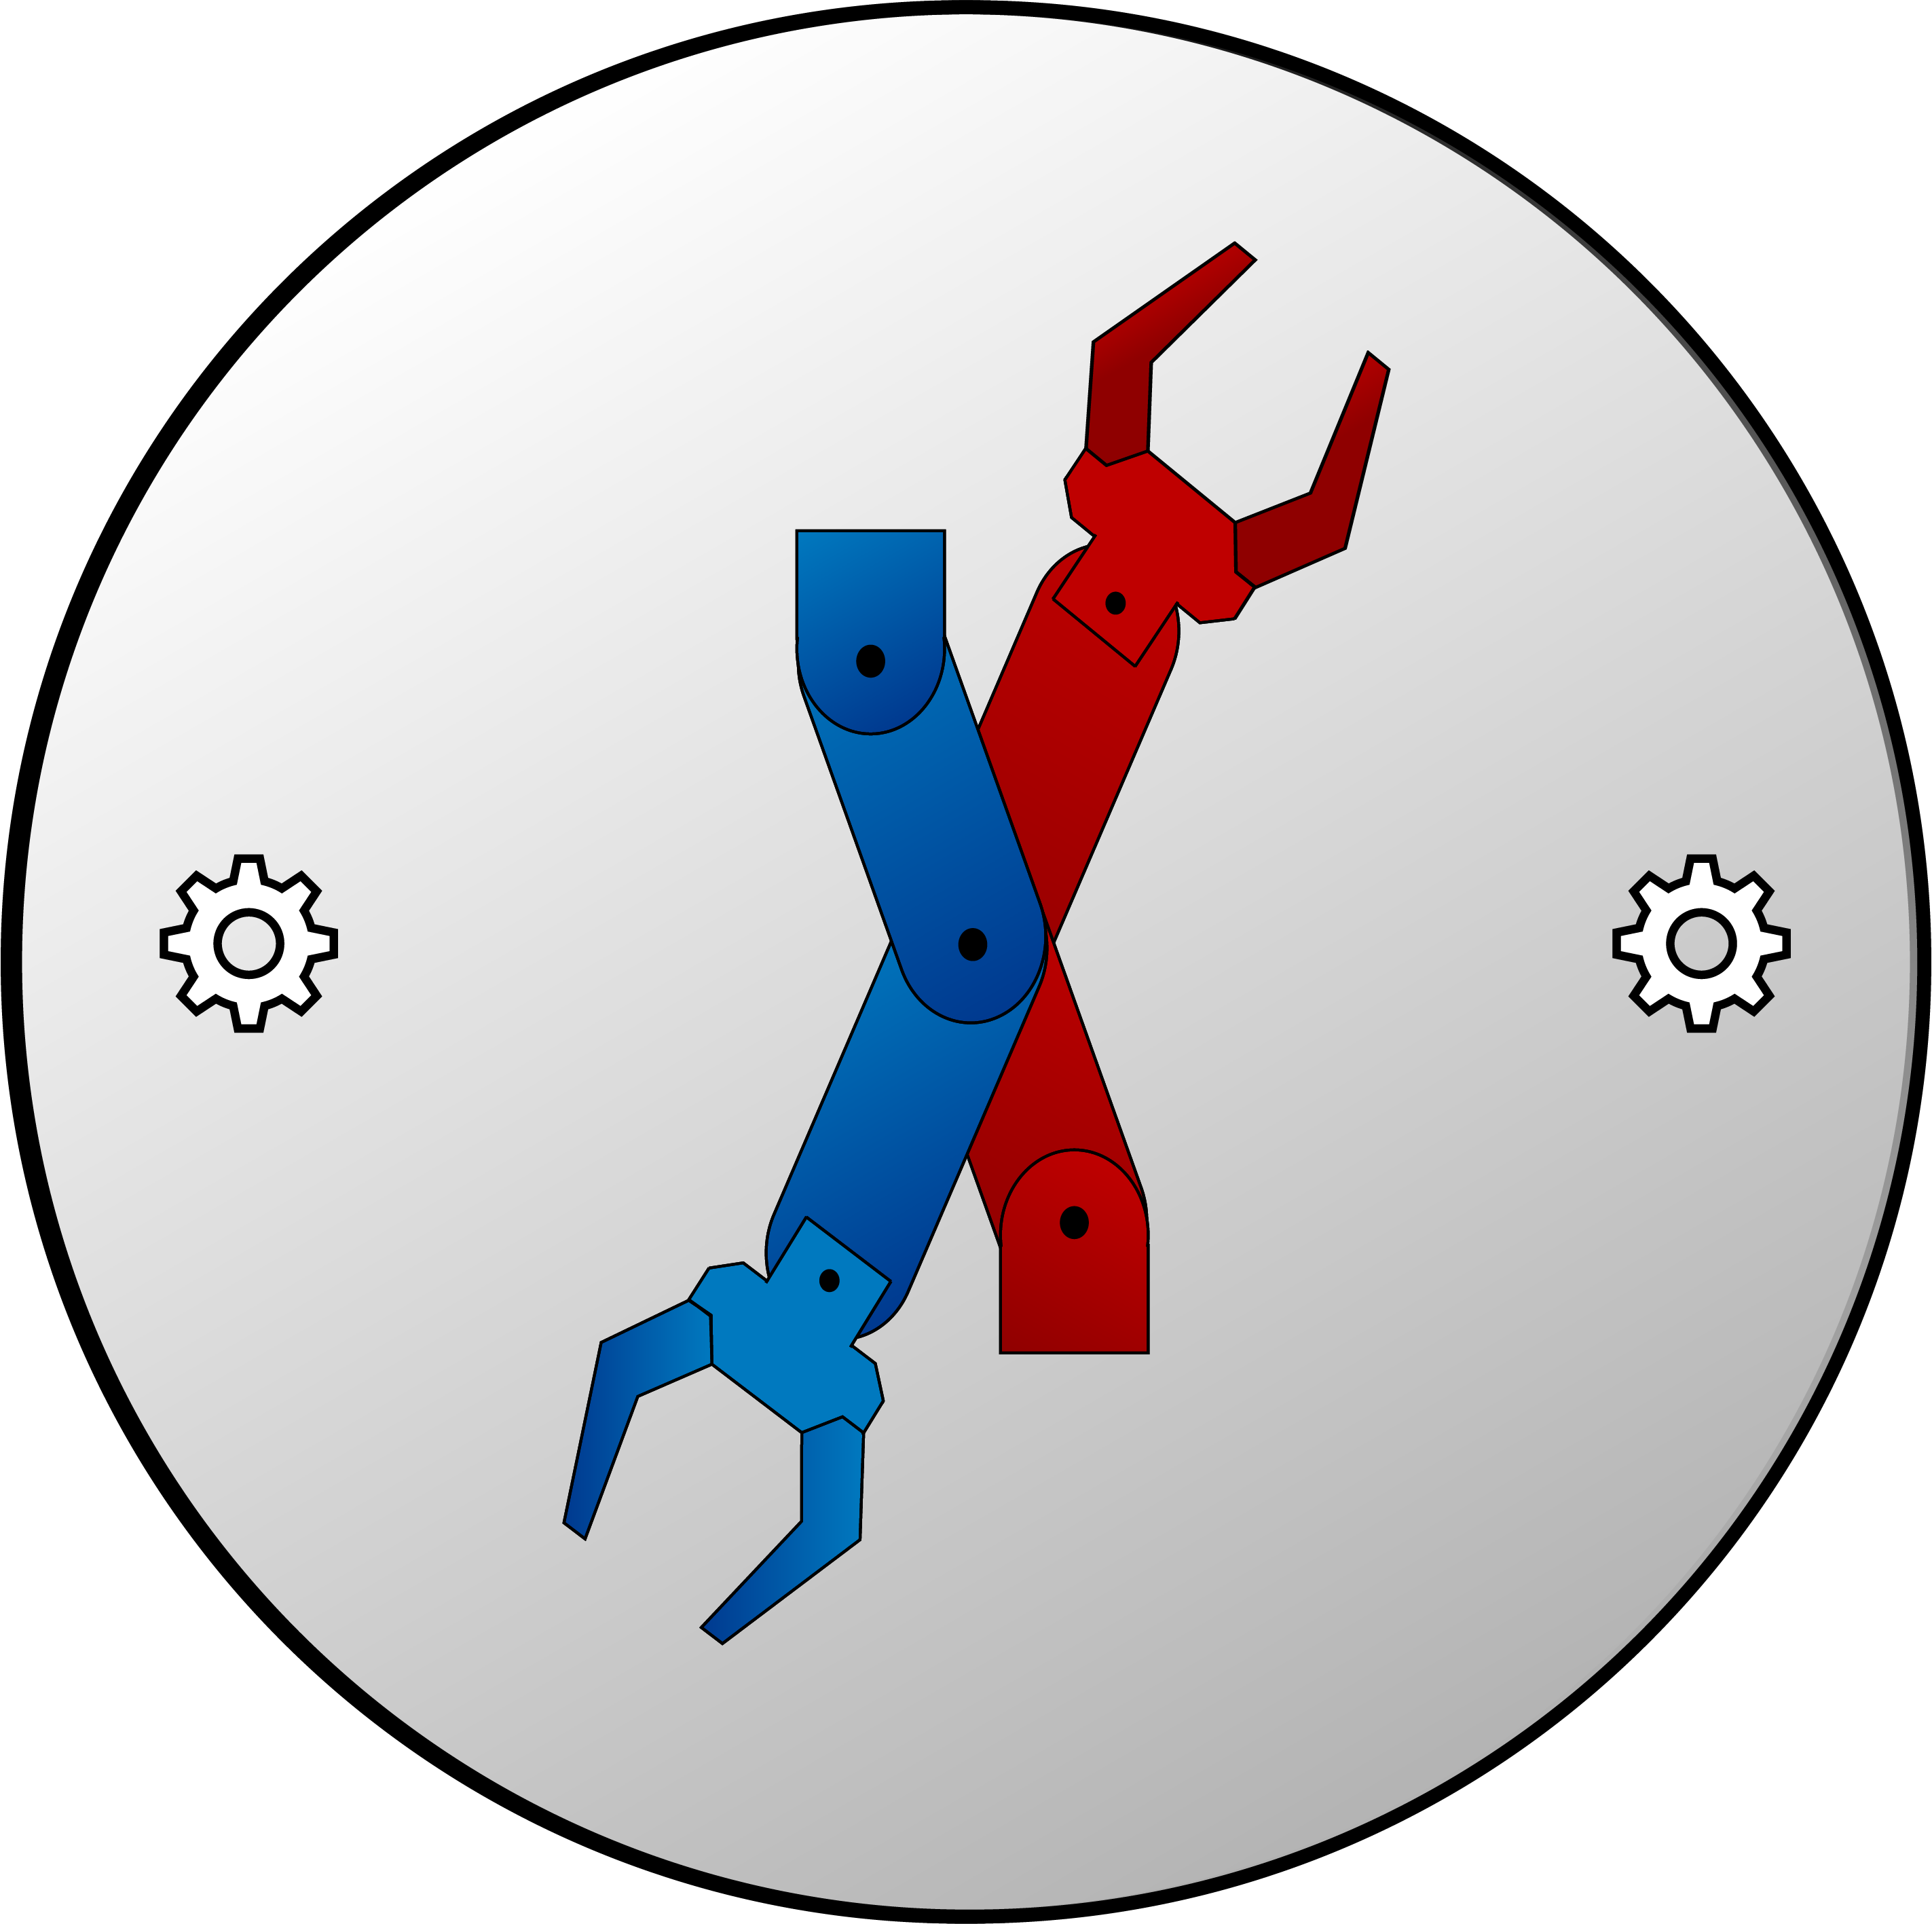
\includegraphics[width=.45\textwidth]{logo}
\vfill
\flushleft
ME 407 \\
Preliminary Design of Robotic Systems \\
Embry-Riddle Aeronautical University \\
\vspace{2ex}
\begin{minipage}[c]{.5\textwidth}
\flushleft

\includegraphics[width=.95\textwidth]{erau}
\end{minipage}%
\begin{minipage}[c]{.5\textwidth}
\flushright

\includegraphics[width=.8\textwidth]{text}
\end{minipage}
\end{titlepage}

\pagenumbering{roman}
% \begin{abstract}
  % Wordy words
% \end{abstract}
{\tableofcontents\let\clearpage\relax\listoffigures\let\clearpage\relax}
\clearpage
\newpage

\section*{List Of Acronyms and Abbreviations}
\begin{tabular}{rl}
  $G$~:&Center of gravity of the bar \\
  $\ell_0$~:& Spring unstretched length  \\
  $\delta$~:& Spring deflection \\
  % $k$~:& Spring constant \\
  % $h_{b}$~:& Distance to bar ($G$) from datum \\
  % $F_s$~:& Force onto bar due to spring\\
  % $A_{n}$~:& Pin reaction in $\theta$ direction\\
  % $A_{t}$~:& Pin reaction in tangential direction \\
  % $\vec{v}_G$~:& Velocity of bar center of gravity\\
  % $\ddot{\theta}$~:& Angular velocity of spring \\
  % $\ddot{\phi}$~:& Angular velocity of bar\\
  % $\ddot{\ell}_s$~:& Radial acceleration of spring \\
\end{tabular}

% \large
% \[
% {}^I_Br_1
% \]
% \normalsize

\newpage

\pagenumbering{arabic}
\section{Introduction}
\section{Requirements}
% \hiddensubsection{Introduction}
Robotics is a fast growing field, yet numerous potential innovators for the discipline are never exposed to it. While many industrial style manipulators are available for commercial applications, their cost is so high that they are not practical for many educational purposes. Schools in rural areas are financially limited and cannot afford a manipulator, nor an instructor who can teach the course due to its complexity. Hence, we propose MEIOSIS robotics: The Manipulator for Educational Institutions with Open Source Integrated Systems. The goal of the project is to produce an inexpensive, rudimentary but capable manipulator that can be purchased as a kit by educators but is available to the general public.
\hiddensubsection{Design Requirements}
In order to create a manipulator that solves the problem stated above, the following requirements must be met.
\hiddensubsection{Hardware}
The following requirements are hardware specific and dictate the physical constraints the system must adhere to.
\subsubsection{The system shall cost the end-user no more than \$1000.}
\subsubsection{The system shall be fully dexterous without being kinematically redundant.}
To create a system with the intention of advancing education, it must be complex enough to encourage higher level problem solving, as well as be capable enough (dexterous) in a broad spectrum of tasks — in the interest of remaining useful in addition to retaining the interest of students.

\subsubsection{The system end effector shall maintain a positional accuracy magnitude of \(\pm 1\) mm and an orientation accuracy of \(\pm 5^{\circ}\) eigen angle from the base frame.}
To ensure that the robot has educational value, the accuracy must be defined so that any desired positions and movements are achieved.

\subsubsection{The system end effector shall maintain a pose repeatability magnitude between 0.1—1.5 mm for the position and \(\pm 4^{\circ}\) eigen angle from the base frame for the orientation.}
This is to ensure a robot that can execute the same movement commands repeatedly and have the same results every time.

\subsubsection{The system’s reachable workspace shall be a hemisphere with a radius of 300-700 mm.}
This workspace will provide enough movement to manipulate objects in order to perform basic tasks.

\subsubsection{The system’s dexterous workspace shall contain a hemispherical shell within the reachable workspace with a thickness of 280 mm.}

\subsubsection{The system shall have a removable end effector capable of picking and placing a low-odor chisel tip Expo dry erase marker.}
This creates a robot capable of performing a variety of basic tasks, which enhances its educational value.

\subsubsection{The system shall be able to write with a low-odor chisel tip Expo dry erase marker.}

\hiddensubsection{Software}
\subsubsection{The system shall be open source.}
This will create an easily obtainable, low cost method of distributing the system’s source code, which may be modified for personal use.

\subsubsection{The system shall be capable of operating given only desired end effector cartesian coordinates specified with respect to the base frame.}
This simplicity makes the system of use to inexperienced users.


% \begin{itemize}
%   \item The system shall cost the end-user no more than \$1000.
%   \item The system shall be fully dexterous without being kinematically redundant.
%   \item The system end-effector shall maintain a positional accuracy magnitude of \(\pm 1\) mm and an orientation accuracy of \(\pm 5^{\circ}\) eigen angle from the base frame.
%   \item The system end-effector shall maintain a pose repeatability magnitude between 0.1 - 1.5 mm for the position and \(\pm 4^{\circ}\) eigen angle from the base frame for the orientation.
%   \item The system’s reachable workspace shall be a hemisphere with a radius of 300-700 mm.
%   \item The system’s dexterous workspace shall contain a hemispherical shell within the reachable workspace with a thickness of 280 mm.
%   \item The system shall have a removable end-effector capable of picking and placing a low-odor chisel tip Expo dry erase marker.
%   \item The system shall be able to write with a low-odor chisel tip Expo dry erase marker.
%   \item The system shall be open source.
%   \item The system shall be capable of operating given only desired end-effector cartesian coordinates specified with respect to the base frame.
% \end{itemize}
\newpage
\section{Conceptual Design}
The terminator T-2000 is a science-fiction spectacle of a robot -- until you see the price. Channeling the inspiration many high school students may have for robotics, MEIOSIS robotics aims to provide an affordable manipulator to educators and enthusiasts. MEIOSIS uses primarily 3-D printed components and easily accessible materials. Among these materials are a Raspberry PI, smart servos and metal tubing. These features create an open-source manipulator accessible to the public to further robotics education.
\hiddensubsection{Physical System Overview}
The physical design of the robotic manipulator will be shown through Figures \emph{\ref{fig:overall}, \ref{fig:base}, \ref{fig:link1},} and \emph{\ref{fig:link2}}.

\begin{figure}[htp]
  \centering
  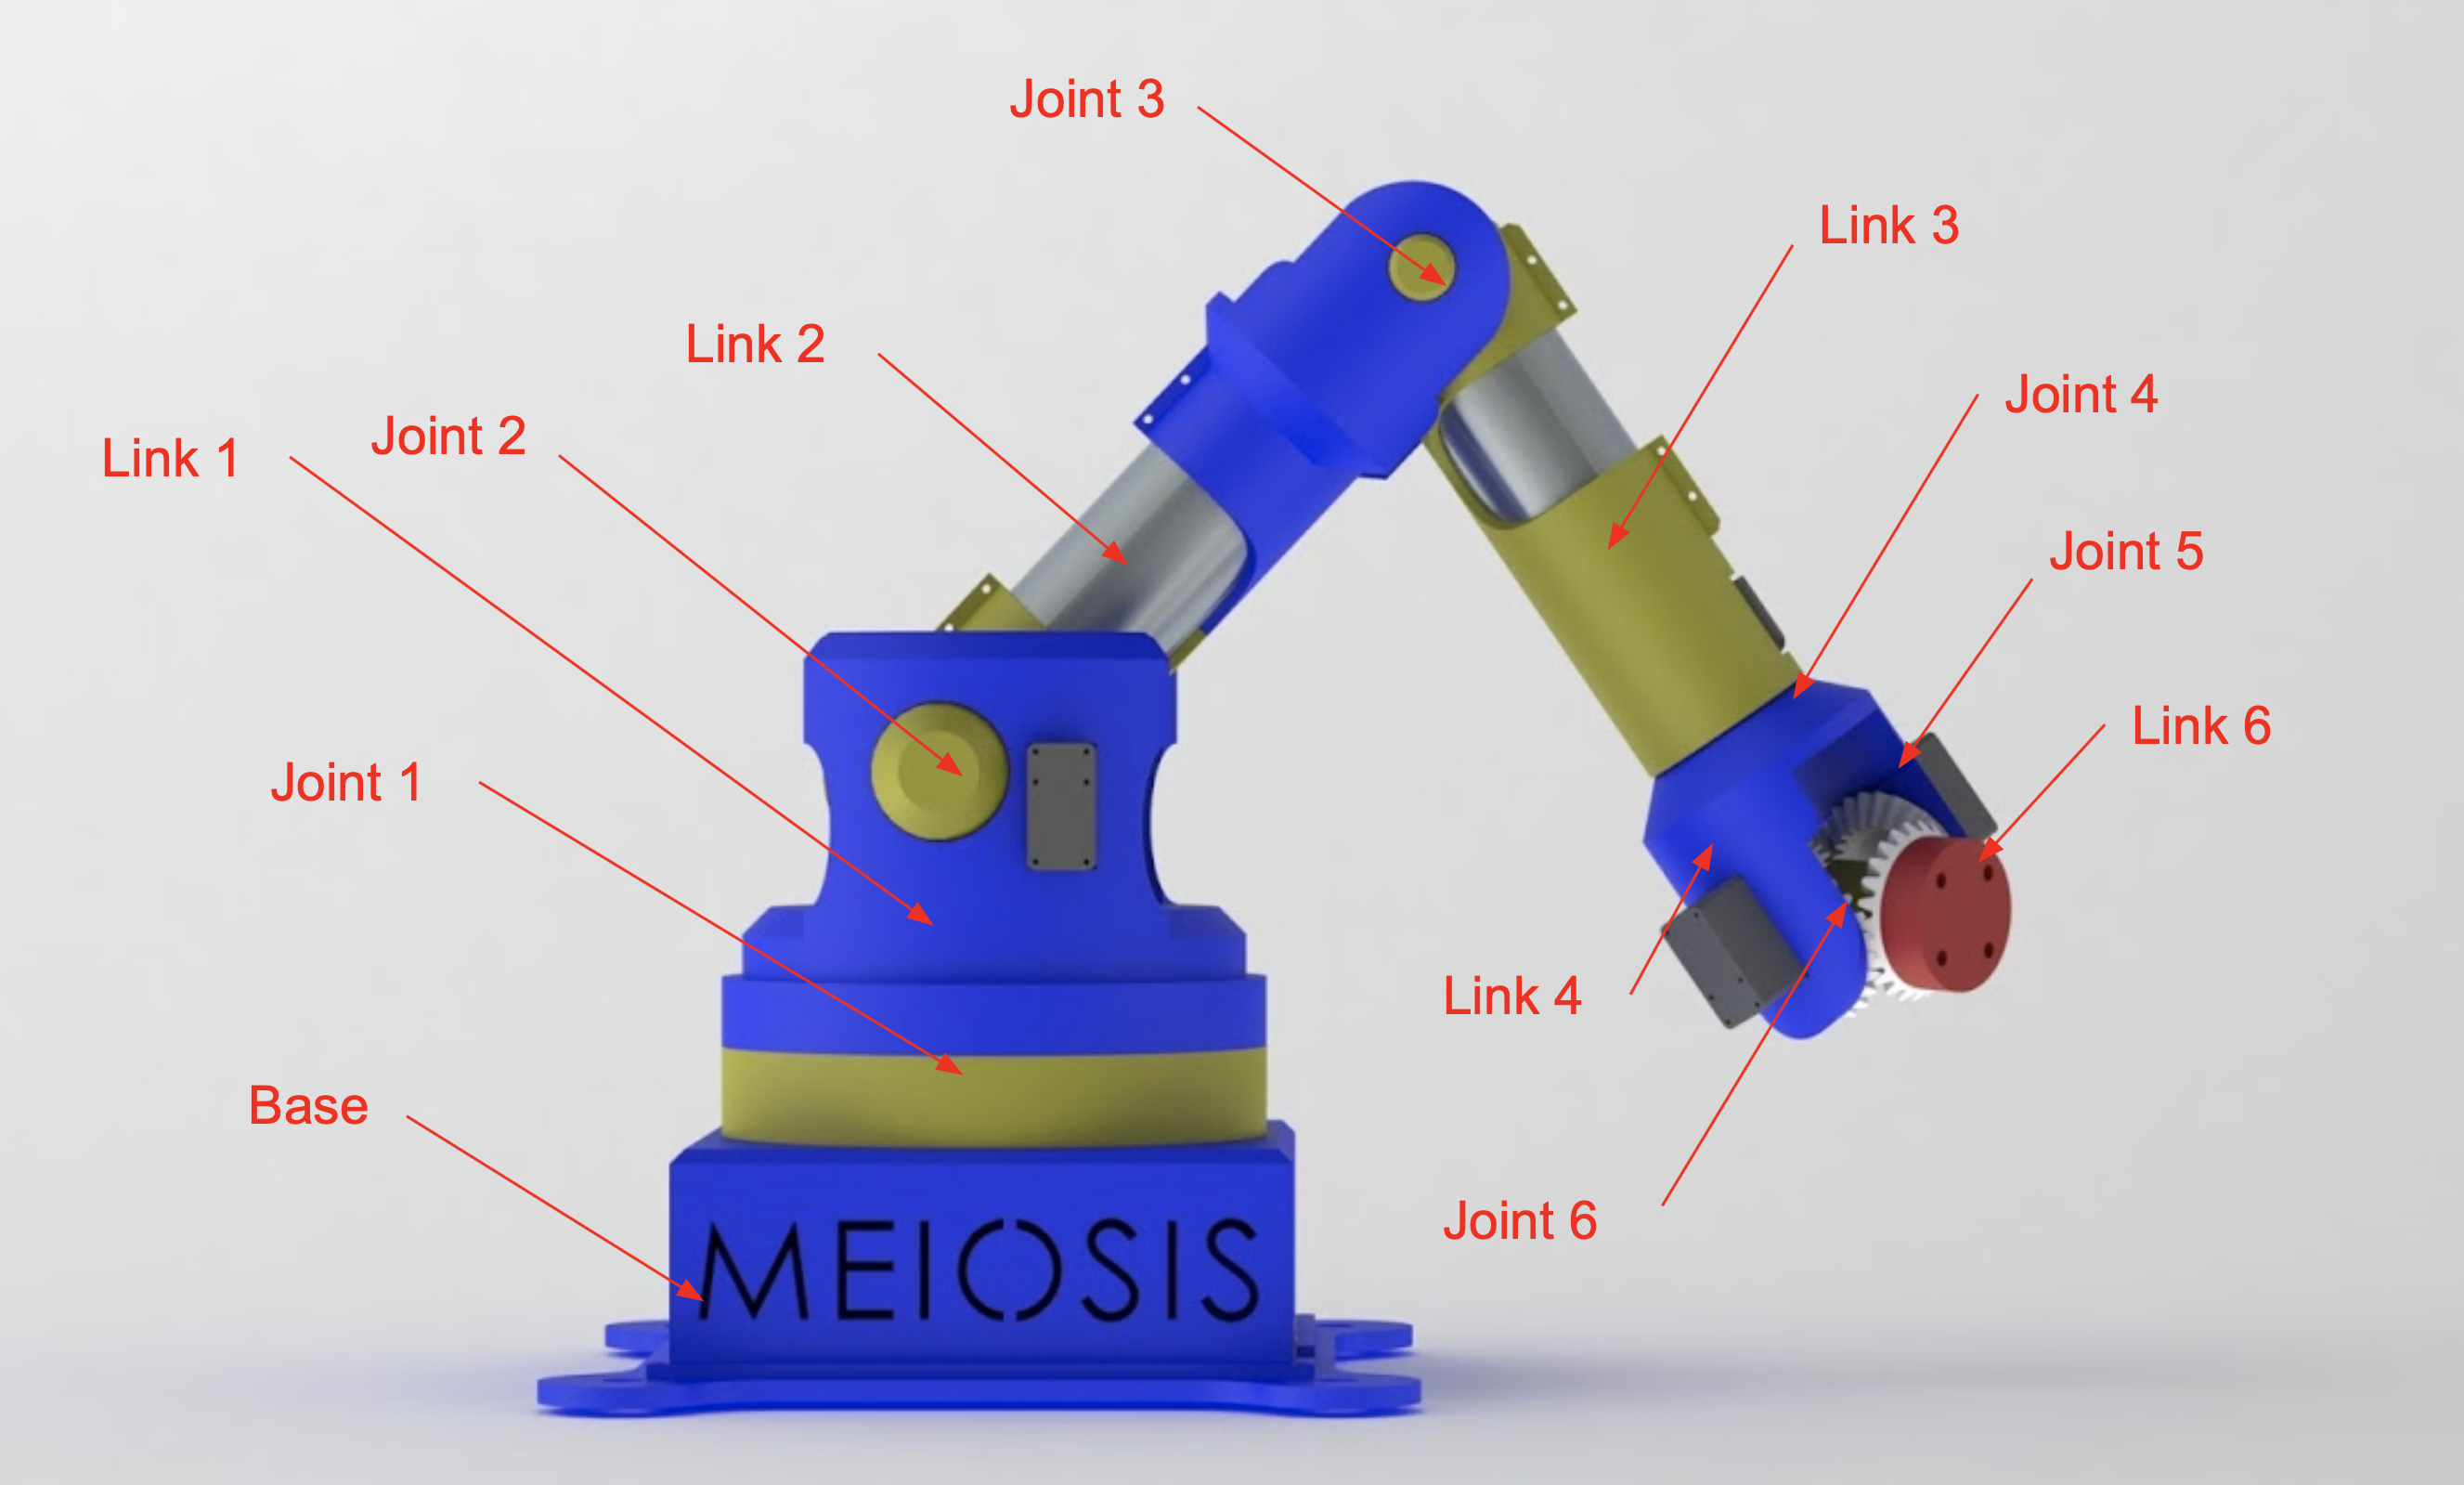
\includegraphics[frame, width=.75\textwidth]{overall_render}
  \caption{Overall System Conceptual Design }
  \label{fig:overall}
\end{figure}

The colored links in \emph{Figure \ref{fig:overall}} distinguish the different joints and links of the manipulator. The overall reach of the robot will be 582.5 mm. This length was chosen to decrease material cost and weight while still satisfying requirement 2.1.2 and 2.1.5, allowing the manipulating to pick and place objects to perform basic tasks. The base of the robot will be made to contain the Raspberry Pi and other electrical components.
\newpage
\subsubsection{Base}
The base of the manipulator will house several of the electronic components, such as the computational system, power supply, and motor controller. A cross section of the base can be seen in \emph{Figure \ref{fig:base}}.
\begin{figure}[htp]
  \centering
  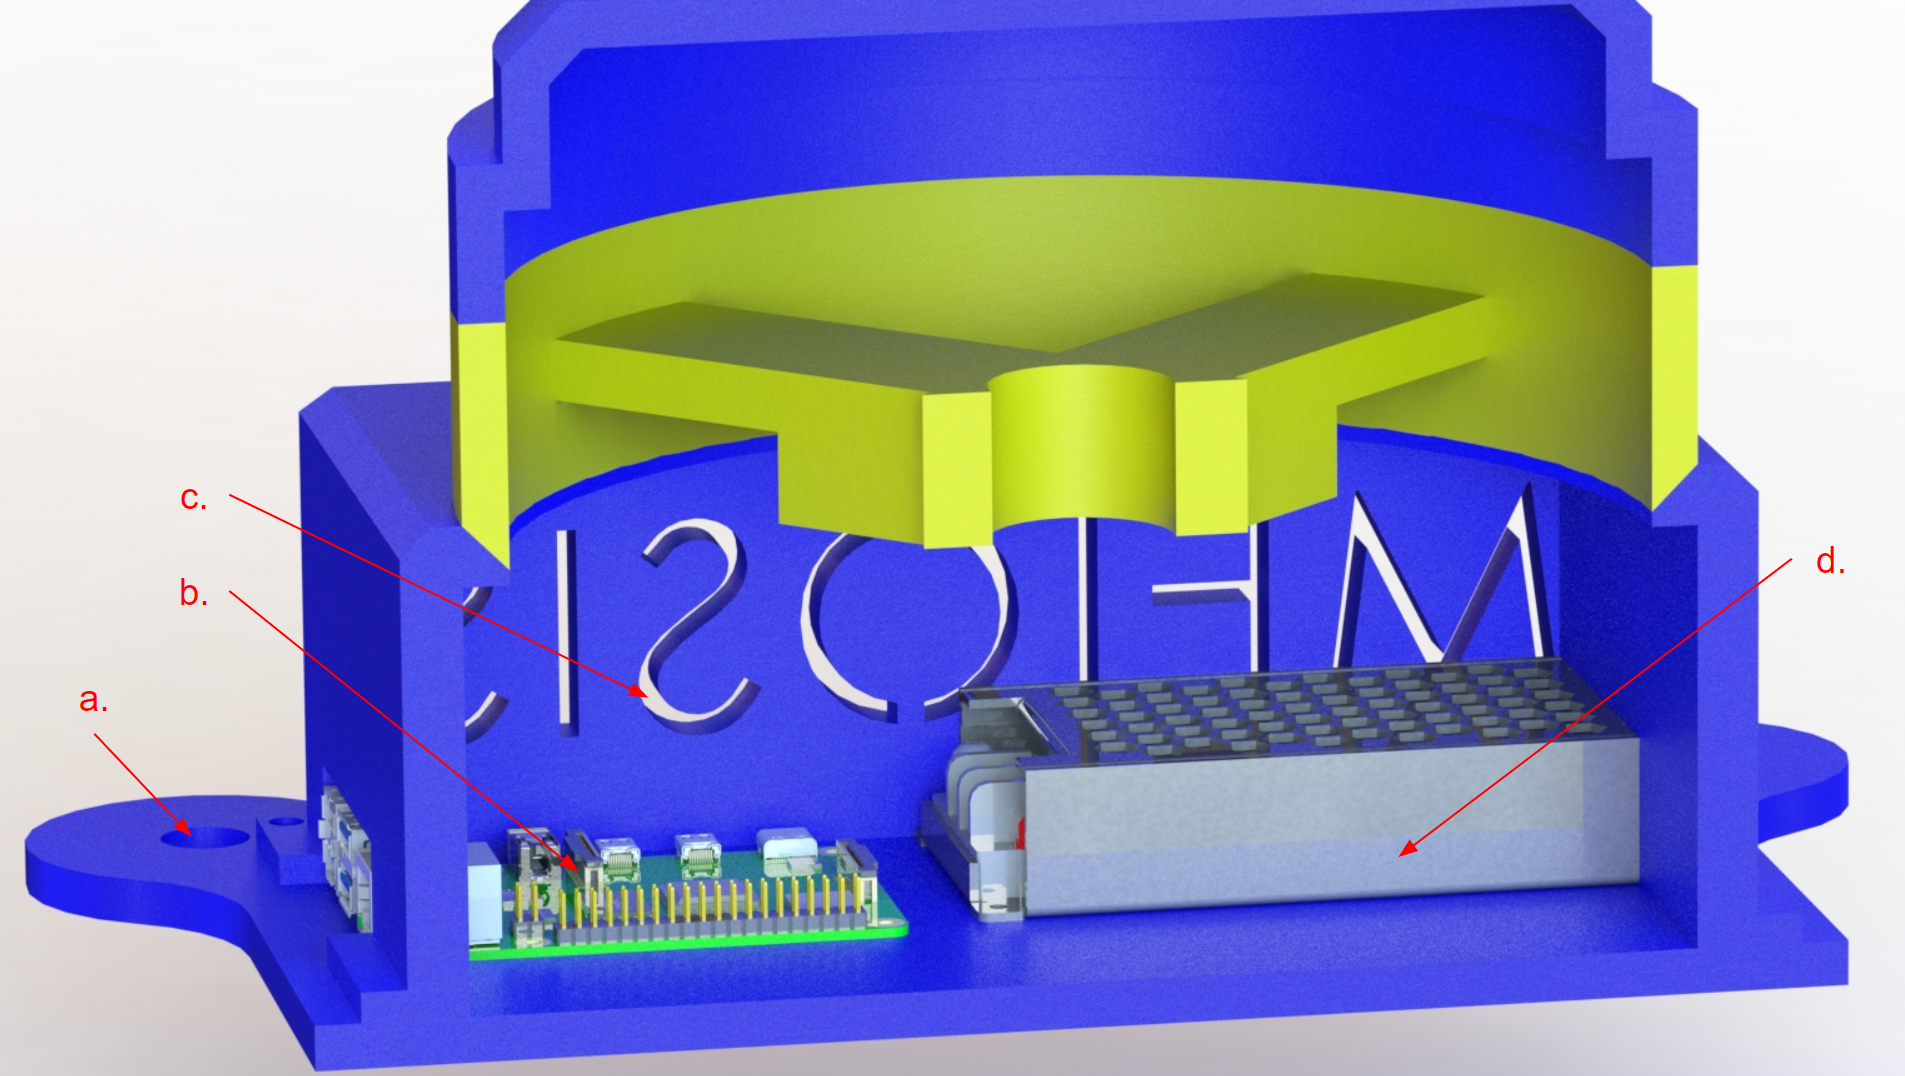
\includegraphics[frame, width=.75\textwidth]{base_callouts}
  \caption{Manipulator Base with Call-outs}
  \label{fig:base}
\end{figure}

From \emph{Figure \ref{fig:base}},
\begin{enumerate}[label=\alph*.]
  \item \emph{Base Supports:}
  The base supports are located at each corner of the base and will allow the base of the manipulator to be securely attached to a variety of surfaces with either standard bolt/fastener hardware or suction cups.
  \item \emph{Computational System:}
  The computational system will be a Raspberry Pi; it will be housed in the base, which allows the Raspberry Pi to be more easily accessible. The primary reason for this system being chosen is to fulfill the budget requirement, 2.1.1. The Raspberry Pi will compute the manipulator's kinematics and command the motors accordingly.
  \item \emph{Airflow Cutouts:}
  The side of the base will have cutouts to allow for airflow through the base; since the power supply is housed inside of the base as well as the computational system, the temperature must be regulated to prevent overheating.
  \item \emph{Power Supply:}
  The power supply will be housed in the base as well; this allows the power supply to be more accessible and therefore more modifiable, so the end-user can easily expand the system to fulfill their needs.
\end{enumerate}
\newpage
\subsubsection{Links}
\emph{Figure \ref{fig:link1}} is an image of the robot that shows the links and their key features.\\
\begin{figure}[htp]
  \centering
  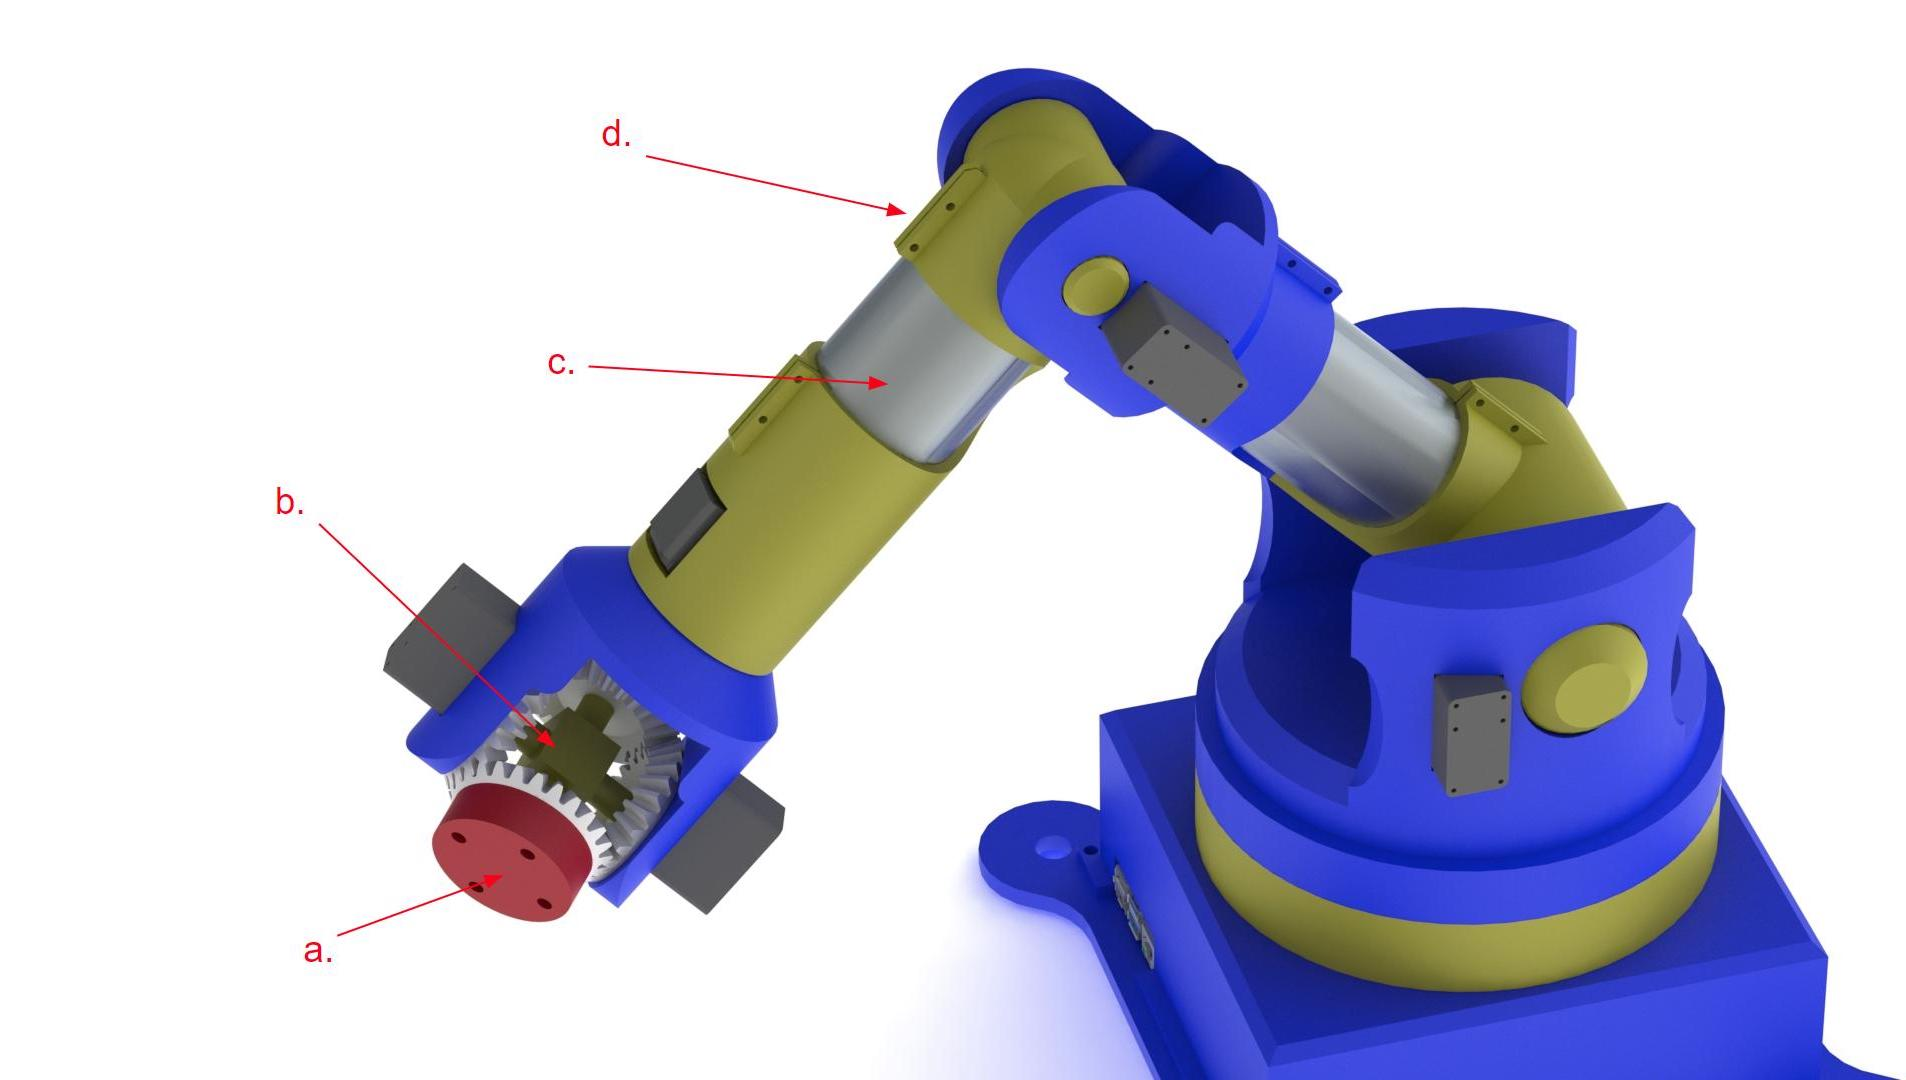
\includegraphics[frame,width=.63\textwidth]{link_callouts}
  \caption{Drawing Showing Key Features of Design}
  \label{fig:link1}
\end{figure} \\
\emph{Figure \ref{fig:link1}} highlights a few of the key features of our design. Call-out a shows the connection point for the end effector. The mountings are the standard used by the Sawyer manipulator. This may be adjusted to accommodate lower cost, more accessible end effectors. Call-out (b) shows the differential gearbox that will be used in the manipulator’s wrist, saving space and weight. The manipulator will have aluminum tubing as support in the links (c) and will be attached to the 3D printed portion of the robot using clamp joints (d) tightened by screws.

\emph{Figure \ref{fig:link2}} is an image of the cross section of link 2 for the manipulator.
\begin{figure}[htp]
  \centering
  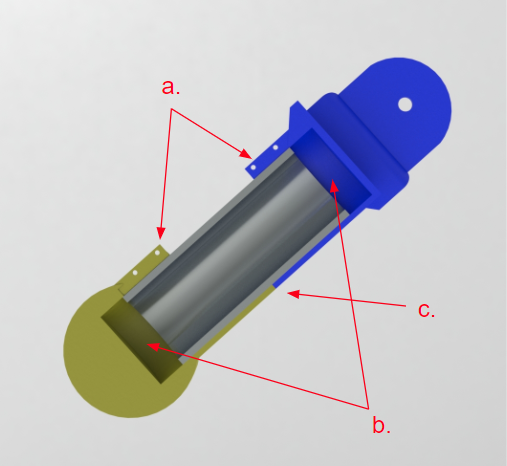
\includegraphics[frame,width=.35\textwidth]{link_cross_section}
  \caption{Drawing Showing Link Cross Section}
  \label{fig:link2}
\end{figure}

The cross section seen in \emph{Figure \ref{fig:link2}} shows the internal design for links two and three. It features two clamps that hold a hollow aluminum bar in place (a) and allows for gaps between the aluminum tube and the 3D printed call-out (b). The proper length will be dictated by the 3D printed guides lining up at call-out (c). This allows for imprecision in the manufacturing of the aluminum tube.

\hiddensubsection{System Functions}
The system can be divided into two subsystems: the electrical and software systems. The electrical subsystem includes the wiring and hardware computational components, power system, actuators with drivers, and sensors. The software subsystem includes the algorithm for the computational system.
\subsection{Electrical}
\emph{Figure \ref{fig:eblock}} is the block diagram for the electrical system of the manipulator.

\begin{figure}[htp]
  \centering
  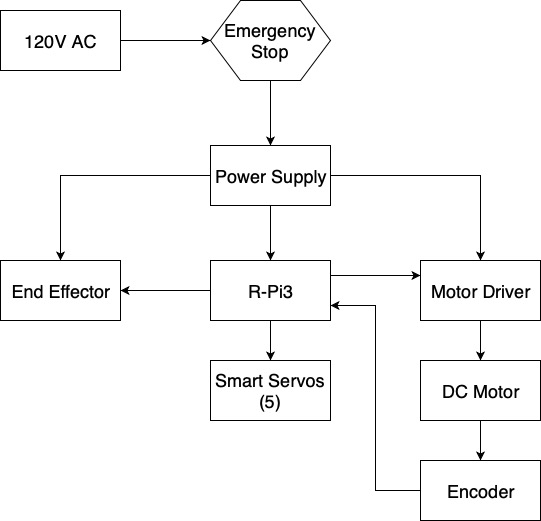
\includegraphics[width=.55\textwidth]{eblock}
  \caption{Electrical System Block Diagram}
  \label{fig:eblock}
\end{figure}

\emph{Figure \ref{fig:eblock}} shows that the electrical systems of the manipulator will be relatively simple. Power is supplied by the 120V AC from standard wall outlets. A power supply will adapt the AC voltage to the required voltages for each component. One component is the Raspberry Pi, which will perform calculations for motor control (described below in software). It will send signals to the DC motor driver and the five smart servos. The smart servos have an on-board controller, so no feedback will be necessary. However, the first joint, between the base and the first link, will be actuated by a DC motor with an encoder to minimize cost.

\hiddensubsection{Software}
\emph{Figure \ref{fig:sblock}} shows the software flowchart for the system.
\begin{figure}[ht]
  \centering
  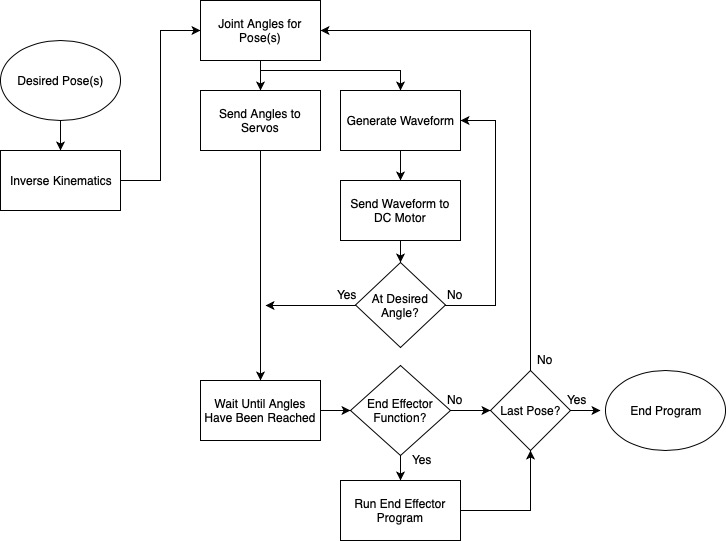
\includegraphics[width=.85\textwidth]{sblock}
  \caption{Software Flowchart}
  \label{fig:sblock}
\end{figure}

Similar to the electrical system, the software is also simple. \emph{Figure \ref{fig:sblock}} shows that the software will receive the desired pose or poses the user would like the manipulator to reach. Then the Raspberry Pi will use inverse kinematics to calculate the necessary joint angles. The wave-forms/desired angles will be sent to the respective drivers/motors, and positional information will be sent back to the Raspberry Pi to adjust the DC motor angle. When the motors have reached their desired pose, the Raspberry Pi will actuate the end effector if it is specified by the user. The system will then check to see if there are any more poses to reach and either repeat the motor control section given the desired angles of the new pose or end program if the last pose has been reached.
\newpage

\section{Specifications}
% \hiddensubsection{Introduction}
\label{sec:intro}
With the intention of making robotics education more accessible, The Manipulator for Educational Institutions with Open Source Integrated Systems (MEIOSIS) intends to provide high school educators and robot enthusiasts with a low cost manipulator. The system should be usable by novice students. It should also be modifiable to create a sustainably increased understanding of robotics. While MEIOSIS may not fully emulate industrial manipulators, it aims to provide more students with access to robotics education. \\
\begin{figure}[htp]
  \centering
  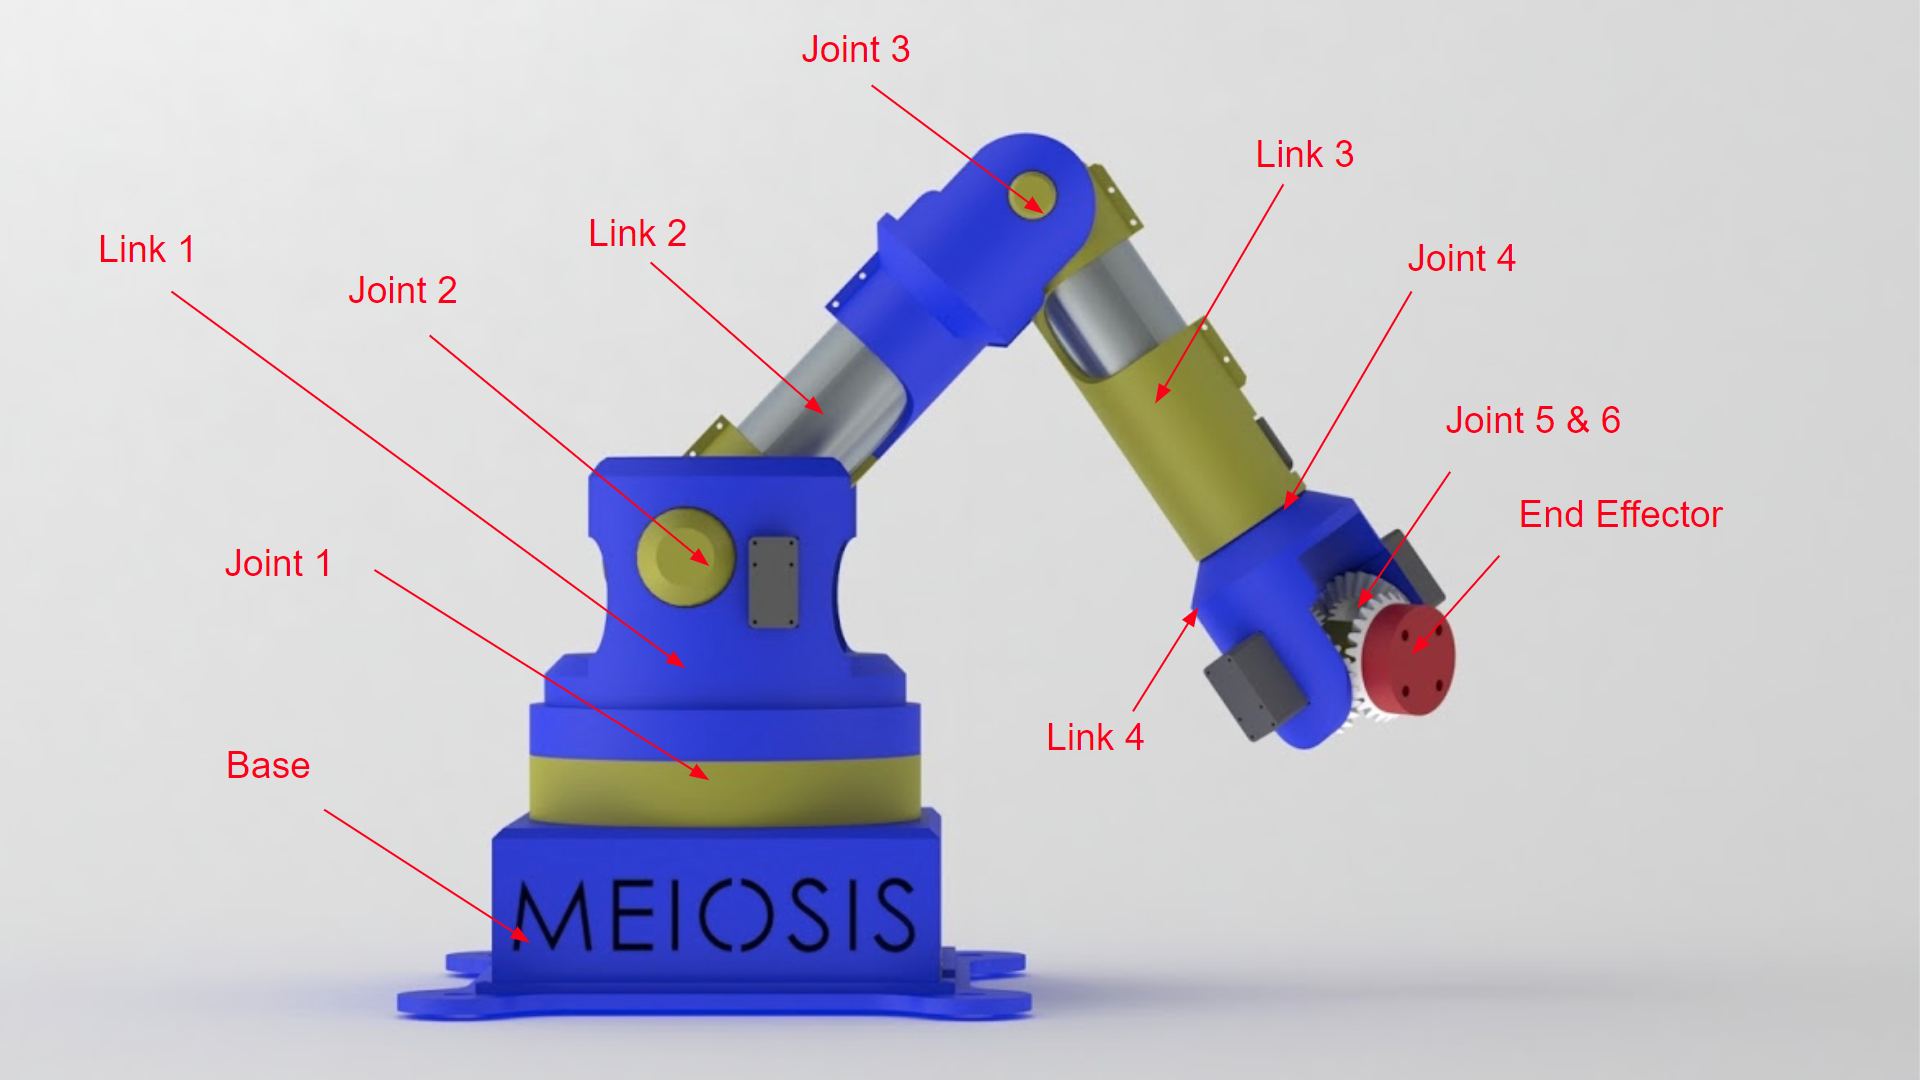
\includegraphics[frame,width=.75\textwidth]{model}
  \caption{Overview of Physical System}
  \label{fig:model}
\end{figure}
\newline
The design seen in \emph{Figure \ref{fig:model}} is based on our conceptual design. It features four links and six joints for rotation and will be referenced throughout this document. The base of the manipulator and end-effector can also be seen in the figure.
\hiddensubsection{Design Requirements}
The specifications of the system are strictly based on the requirements defined previously. The requirements are divided into two primary categories, hardware and software.
\vspace{-\baselineskip}
\hiddensubsection{Hardware}
The following requirements and specifications are hardware specific and dictate the physical constaints the system must adhere to.
\vspace{-\baselineskip}
\subsubsection{The system shall cost the end-user no more than \$1000.}
\begin{enumerate}
  \item \textit{The cost for the MEIOSIS team to develop the manipulator shall cost no more than \$800.}
\end{enumerate}

\subsubsection{The system shall be fully dexterous without being kinematically redundant.}
\begin{enumerate}
\item \textit{The system shall consist of six rotational joints connected by four links. The last three joints will create a spherical wrist.}
\end{enumerate}
As defined \cite{robo}, “A manipulator having more than six DOF is referred to as a kinematically redundant manipulator (5).” A manipulator with less than six degrees of freedom will not be fully dexterous within it's workspace. \emph{Figure \ref{fig:zero}} (see subsection \ref{sec:zero}, p. \pageref{fig:zero}) shows a six degree-of-freedom rotary manipulator with it's coordinate frames in zeroed positions. The joint and link locations are seen in \emph{Figure \ref{fig:model}} (see section \ref{sec:intro}, p. \pageref{sec:intro}).
\begin{enumerate}[resume]
\item \textit{The system shall have no link offsets.}
\end{enumerate}
Link offsets as seen in \emph{Figure \ref{fig:offset}} are commonly used to avoid singularities. However, having a link offset prevents the manipulator's dexterous workspace from being a complete hemispherical shell.

\begin{figure}[htp]
  \centering
  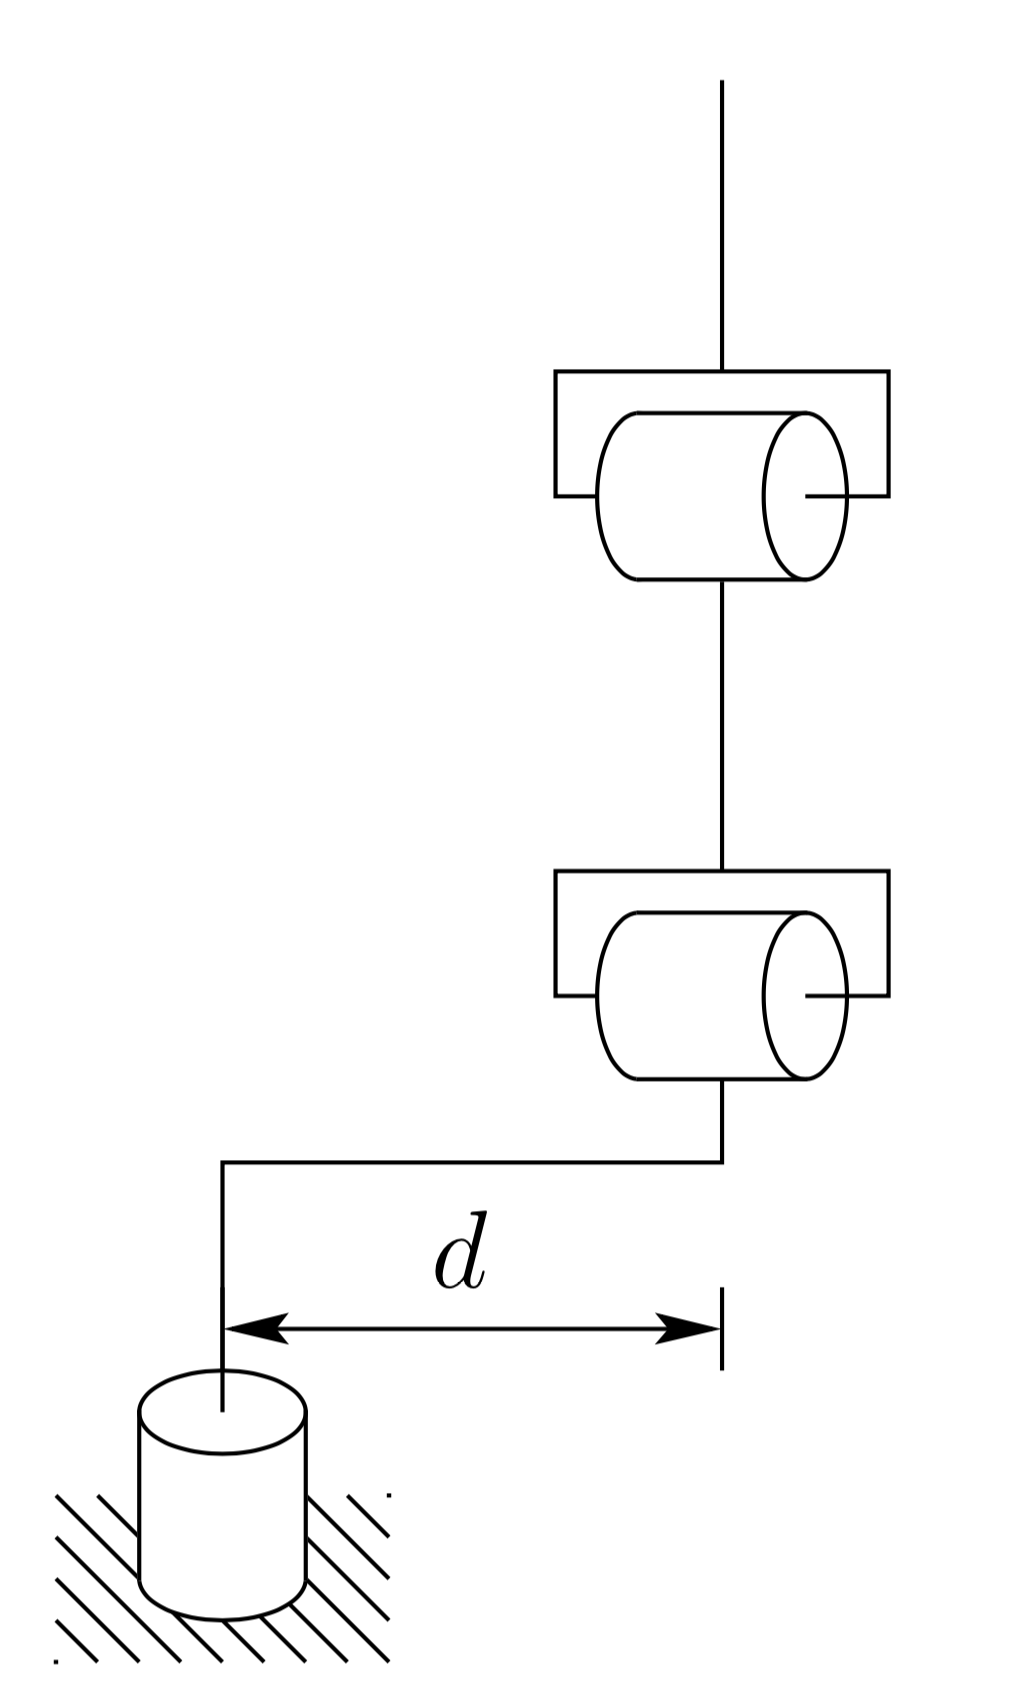
\includegraphics[width=.25\textwidth]{offset}
  \caption[Elbow Manipulator Configuration with Link Offset]{Elbow Manipulator Configuration with Link Offset \cite{robo}}
  \label{fig:offset}
\end{figure}
As shown in \emph{Figure \ref{fig:offset}}, the line directly above the first joint of the manipulator is offset such that the axes of the other joints are unable to become collinear with the base axis; this prevents singularity but causes a void in the detxterous workspace.
\subsubsection{The system end effector shall maintain a positional accuracy magnitude of \(\pm 1\) mm and an orientation accuracy of \(\pm 5^{\circ}\) eigen angle from the base frame.}
To ensure that the robot has educational value, the accuracy must be defined so that any desired positions and movements are achieved.
\begin{enumerate}
  \item \textit{The system shall accommodate a process in which the end user can calibrate the end effector position and orientation to within 0.5 mm and 1 degree of the manipulator’s precision.}
\end{enumerate}
The addition of a calibration process allows the removal of any systematic errors, such as drift. The theoretical limit of the calibration process is the difference between the precision and accuracy metrics of the system.
\subsubsection{The system end effector shall maintain a pose repeatability magnitude between 0.1—1.5 mm for the position and \(\pm 4^{\circ}\) eigen angle from the base frame for the orientation.}
\begin{enumerate}
  \item \textit{Joint one and two of the system shall possess an angle error of no more than .025 degrees.}
\end{enumerate}
Being that joint one and two are the first two rotational elements in the system, their error will propagate the most to the end effector's position.
\begin{enumerate}[resume]
  \item \textit{Joint three of the system shall possess an angle error of no more than .03 degrees.}
\end{enumerate}
Since joint three is closer to the end effector it's error will not propagate as severely throughout the system.
\begin{enumerate}[resume]
  \item \textit{Joints four, five, and six shall possess an angle error of no more than .29 degrees.}
\end{enumerate}
The spherical wrist is the closest to the end effector's final position and therefore has the least error propagation.

\subsubsection{The system’s reachable workspace shall be a hemisphere with a radius of 300-700 mm.}
This workspace will provide enough movement to manipulate objects in order to perform basic tasks.
\begin{enumerate}
  \item \textit{The length of link one, two, three, four, and the wrist shall be 220.8 mm, 250 mm, 200 mm, 80 mm, and 52.5 mm respectively.}
\end{enumerate}
  This results in a total height of 220.8 mm with a total reach of 582.5 mm in the zeroed configuration as shown in the configuration represented in \emph{Figure \ref{fig:zero}}.

\subsubsection{The system’s dexterous workspace shall contain a hemispherical shell within the reachable workspace with a thickness of 280 mm.}\label{sec:zero}
This workspace will provide enough movement to manipulate objects in order to perform basic tasks. 280mm is slightly greater than the length of letter paper.
\begin{enumerate}
  \item \textit{The rotational limit of joint one, two, three, four, five, and six shall be \(\pm180^{\circ}\), \(-9.7^{\circ}\) to \(177.5^{\circ}\), \(-150.6^{\circ}\) to \(-19.3^{\circ}\), \(\pm180^{\circ}\), \(-180^{\circ}\) to \(-1.6^{\circ}\), and \(\pm180^{\circ}\) respectively.}
\end{enumerate}
The angles stated are with respect to the kinematic model shown in \emph{Figure \ref{fig:zero}}. To be fully dexterous within our 280 mm dexterous workspace the manipulator must have the joint angles specified above. The joint limitations were calculated by iteratively verifying the orientation about every point within the quarter hemisphere cross section seen in \emph{Figure \ref{fig:dex}} (see Appendix, p. \pageref{sec:app}).
  \begin{figure}[htp]
    \centering
    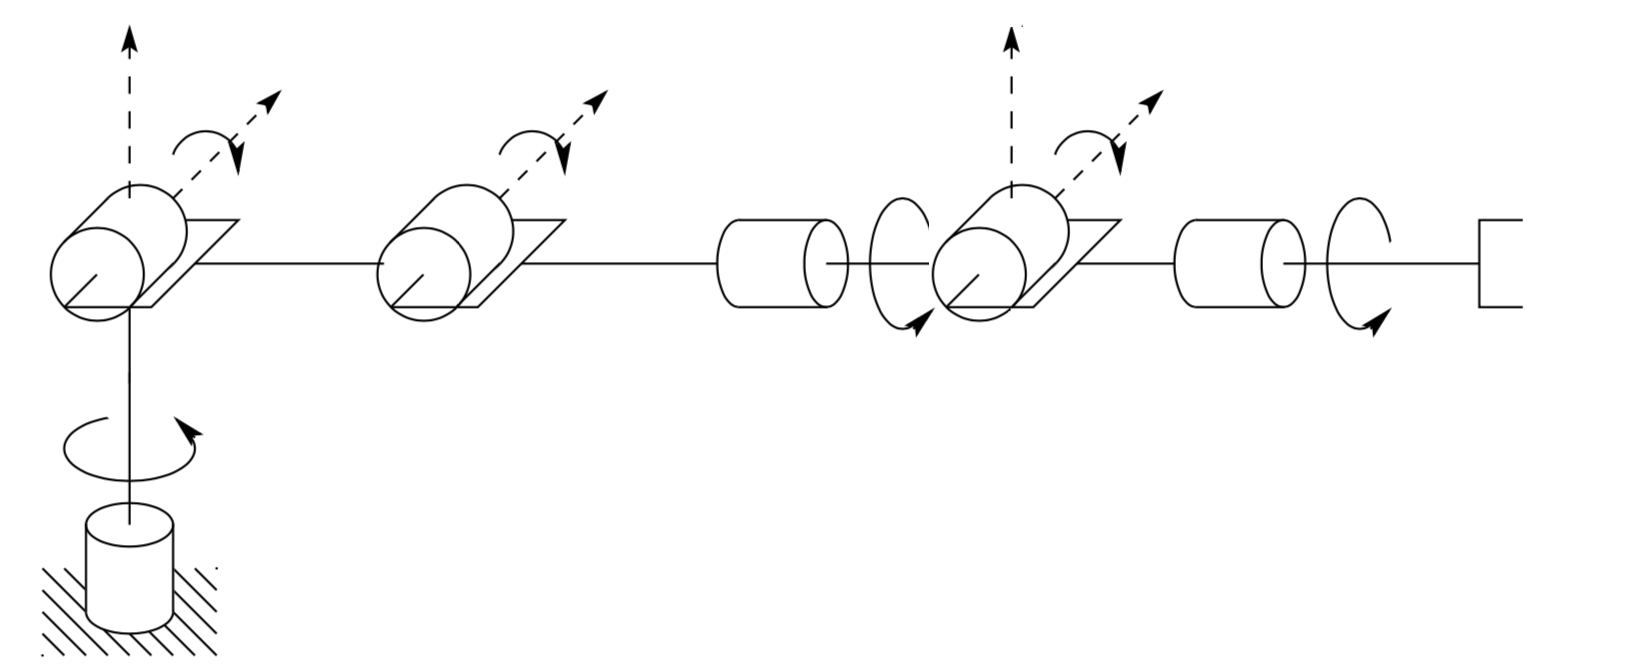
\includegraphics[width=.75\textwidth]{zero}
    \caption[Kinematic Model Representing Zeroed Configuration]{Kinematic Model Representing Zeroed Configuration \cite{robo}}
    \label{fig:zero}
  \end{figure}
\subsubsection{The system shall have a removable end effector capable of picking and placing a low-odor chisel tip Expo dry erase marker.}
This creates a robot capable of performing a variety of basic tasks, which enhances its educational value.
\begin{enumerate}
  \item \textit{The system shall use a parallel gripper that can close to 18mm.}
\end{enumerate}
The diameter of a low-odor chisel tip Expo dry erase marker is approximately 18 mm.
\begin{enumerate}[resume]
  \item \textit{The end effector shall attach to the manipulator using screws configured in a pattern that can accommodate a Dynamixel AX-12A servo.}
\end{enumerate}
It is expected that a majority of end effector styles will have to accommodate for a servo to facilitate actuation, therefore a pattern was chosen to standardize the mounting.


\subsubsection{The system shall be able to write with a low-odor chisel tip Expo dry erase marker.}
\begin{enumerate}
  \item \textit{The end effector shall be able to support 0.004 Newton meter moments about the axes normal to its gripping surfaces.}
\end{enumerate}
  The coefficient of friction between the Expo marker and paper can be approximated and given the weight of an Expo marker the approximate grip strength of the end effector can be calculated.
\hiddensubsection{Software}
The following requirements and specifications are software specific and determine the attributes of the operating system.
\subsubsection{The system shall be open source.}
This will create an easily obtainable, low cost method of distributing the system’s source code, which may be modified for personal use.
\begin{enumerate}
  \item \textit{The software shall be hosted publicly on an online repository and maintain an MIT license for distribution.}
\end{enumerate}
  This allows the end-user to freely download and modify the code without licensing. The MIT license disregards any legal obligation to code upkeep and documentation by the original author.

\subsubsection{The system shall be capable of operating given only desired end effector cartesian coordinates specified with respect to the base frame.}
\begin{enumerate}
  \item \textit{The system shall have a user interface capable of accepting the end-effector’s desired cartesian position and Euler angle orientation as a six element row vector.}
\end{enumerate}
  The system software interface facilitates an untrained user to operate without the advanced knoledge of the system's kinematics.
\begin{enumerate}[resume]
  \item \textit{The system shall be capable of performing floating point arithmetic.}
\end{enumerate}
The solution for the inverse kinematics requires the ability to perform high level arithmetic with little error.


% \begin{itemize}
%   \item The cost for the MEIOSIS team to develop the manipulator shall be no more than \$800.
%   \item The system shall consist of six rotational joints connected by four links. The last three joints will create a spherical wrist.
%   \item The system shall have no link offsets.
%   \item The system shall accommodate a process in which the end user can calibrate the end-effector's position and orientation to within 0.5 mm and 1 degree of the manipulator’s precision.
%   \item Joints one and two of the system shall possess an angular error of no more than .025 degrees.
%   \item Joint three of the system shall possess an angle error of no more than .03 degrees.
%   \item Joints four, five, and six shall possess an angle error of no more than .29 degrees.
%   \item The length of link one, two, three, four, and the wrist shall be 220.8 mm, 250 mm, 200 mm, 80 mm, and 52.5 mm respectively.
%   \item The rotational limit of joint one, two, three, four, five, and six shall be \(\pm180^{\circ}\), \(-9.7^{\circ}\) to \(177.5^{\circ}\), \(-150.6^{\circ}\) to \(-19.3^{\circ}\), \(\pm180^{\circ}\), \(-180^{\circ}\) to \(-1.6^{\circ}\), and \(\pm180^{\circ}\) respectively.
%   \item The system shall use a gripper that can close to 18mm.
%   \item The end-effector shall attach to the manipulator using screws configured in a pattern that can accommodate a Dynamixel AX-12A servo.
%   \item The end-effector shall be able to support 0.004 Newton meter moments about the axes normal to its gripping surfaces.
%   \item The software shall be hosted publicly on an online repository and maintain an MIT license for distribution.
%   \item The system shall have a user interface capable of accepting the end-effector’s desired cartesian position and Euler angle orientation as a six element row vector.
%   \item The system shall be capable of performing floating point arithmetic.
% \end{itemize}


\newpage
\section{Preliminary Design}
\subsection{CAD}
\newpage
%------------------------------------------------------------------------------%
% FK
%------------------------------------------------------------------------------%
\subsection{Forward Kinematics}
The forward kinematics of the manipulator are described by the equations below, where the reference coordinate frames are given by Figure (\ref{fig:coords}).
\begin{figure}[htp]
  \centering
  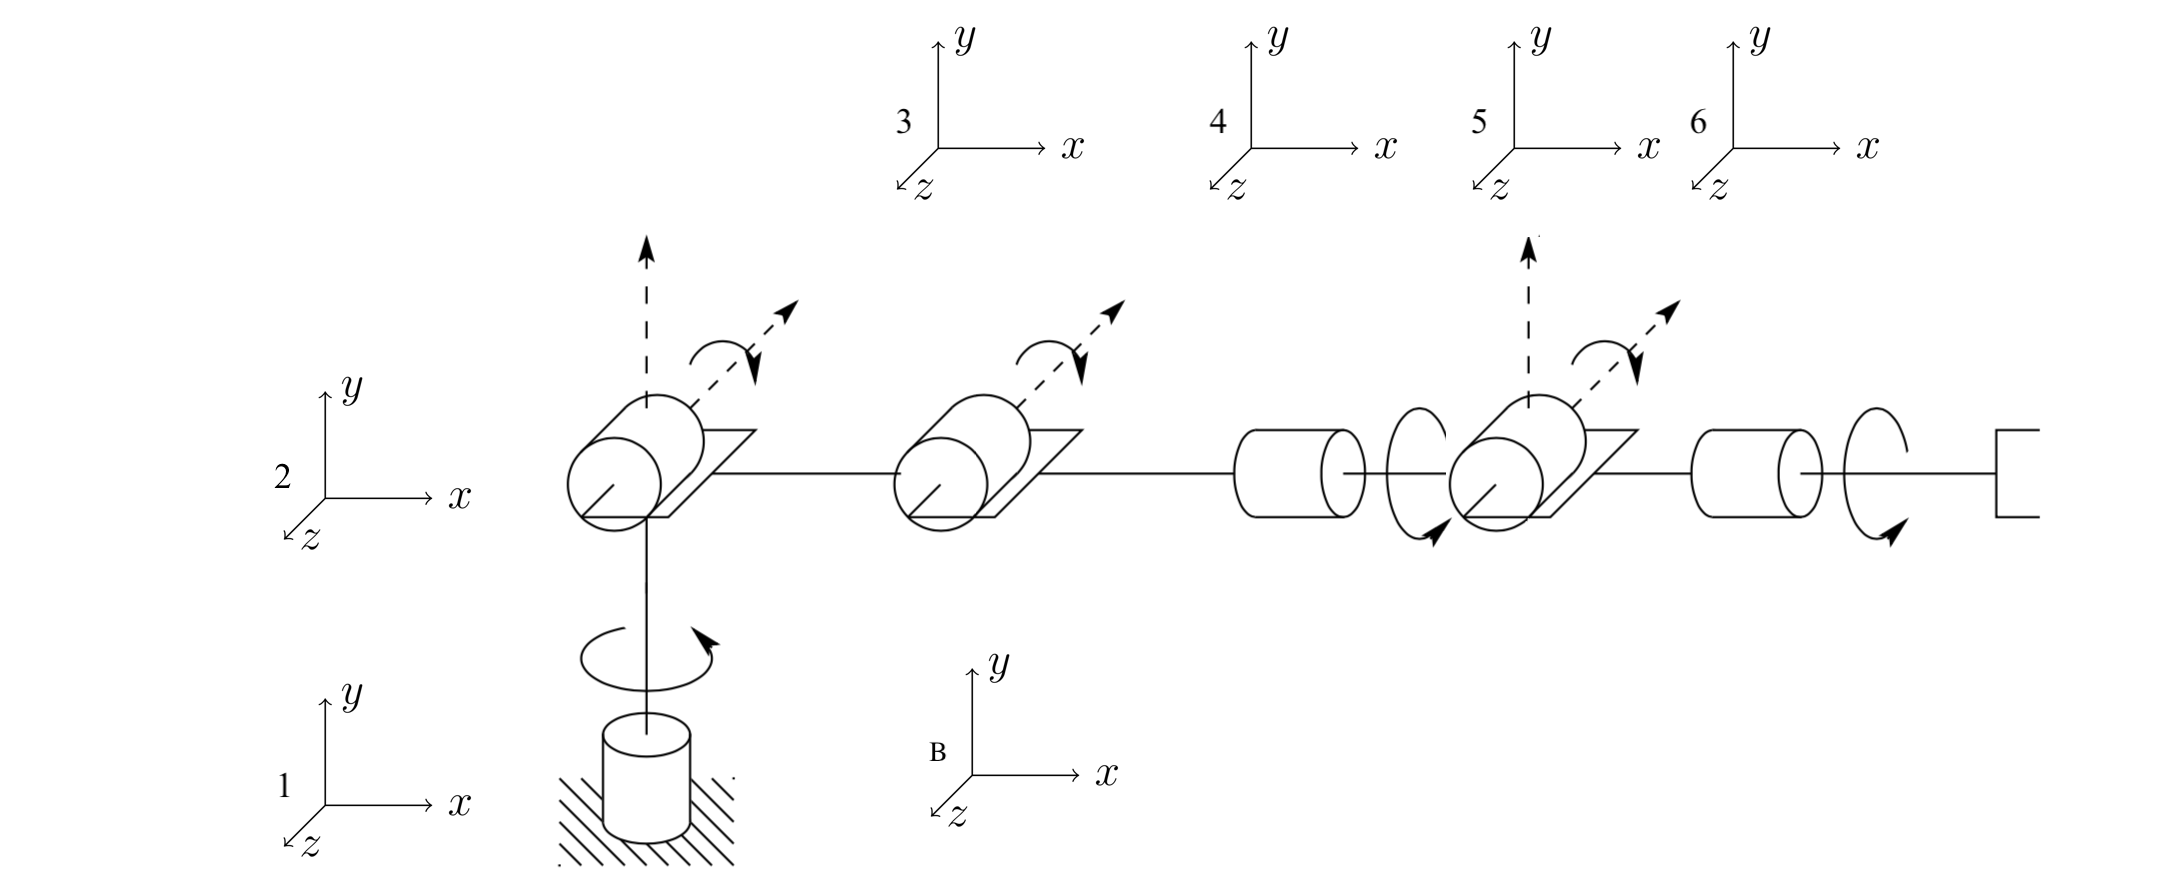
\includegraphics[width=.9\textwidth]{zero2}
  \caption{Coordinate Systems}
  \label{fig:coords}
\end{figure}

Given the lengths of each of the manipulator links,
\[
\begin{aligned}
  ^I_Br_1 = \begin{bmatrix} 0\\0\\ \ell_b\end{bmatrix} & \quad
  ^1_1r_2 = \begin{bmatrix} 0\\0\\ \ell_1\end{bmatrix} & \quad
  ^2_2r_3 = \begin{bmatrix} 0\\\ell_2\\ 0\end{bmatrix} & \quad
  ^3_3r_4 = \begin{bmatrix} 0\\\ell_3\\ 0\end{bmatrix} & \quad
  ^4_4r_5 = \begin{bmatrix} 0\\\ell_4\\ 0\end{bmatrix} & \quad
  ^5_5r_6 = \begin{bmatrix} 0\\\ell_5\\ 0\end{bmatrix} & \quad
\end{aligned}
\]
The position of each link relative to the inertial frame is given as:
\[
\begin{aligned}
^I_Br_1 &= {}_Br_1 &\quad
^I_Br_2 &= r_1 + {}^IT_1 {}^1_1r_2 &\quad
^I_Br_3 &= r_2 + {}^IT_2 {}^2_2r_3 \\
^I_Br_4 &= r_3 + {}^IT_3 {}^3_3r_4 &\quad
^I_Br_5 &= r_4 + {}^IT_4 {}^4_4r_5 &\quad
^I_Br_6 &= r_5 + {}^IT_5 {}^5_5r_6
\end{aligned}
\]

\[
\begin{aligned}
  ^I_Br_1 =&
  \begin{bmatrix}
    0\\ 0\\ \ell_b
  \end{bmatrix} & \quad
  ^I_Br_2 =
  \begin{bmatrix}
    0\\ 0\\ \ell_b + \ell_1
  \end{bmatrix} & \quad
  ^I_Br_3 =
  \begin{bmatrix}
    -\ell_2c_{\theta_2}s_{\theta_1}\\
    \ell_2c_{\theta_{12}}\\
    \ell_b+\ell_1+\ell_2s_{\theta_2}
  \end{bmatrix} & \quad
  ^I_Br_4 =
  \begin{bmatrix}
    -s_{\theta_1}(\ell_3c_{\theta_{23}} + \ell_2c_{\theta_2}) \\
    c_{\theta_1}(\ell_3c_{\theta_{23}} + \ell_2c_{\theta_2}) \\
    \ell_1 + \ell_b + \ell_3s_{\theta_{23}} + \ell_2s_{\theta_2}
  \end{bmatrix} \\
\end{aligned}
  \]
  \[
  ^I_Br_5 =
  \begin{bmatrix}
    -s_{\theta_1}(\ell_3c_{\theta_{23}} + \ell_4c_{\theta_{23}} + \ell_2c_{\theta_2}) \\
    c_{\theta_1}(\ell_3c_{\theta_{23}} + \ell_4c_{\theta_{23}} + \ell_2c_{\theta_2}) \\
    \ell_1 + \ell_b + \ell_3s_{\theta_{23}} + \ell_4s_{\theta_{23}} + \ell_2s_{\theta_2}
  \end{bmatrix}
  \]
  \[
  ^I_Br_6 =
  \begin{bmatrix}
  \begin{aligned}
      &\ell_5c_{\theta_1}s_{\theta_4}s_{\theta_5} - \ell_4c_{\theta_{23}}s_{\theta_1} - \ell_2c_{\theta_2}s_{\theta_1} - \ell_5c_{\theta_{23}}c_{\theta_5}s_{\theta_1} - \ell_3c_{\theta_{23}}s_{\theta_1} \\
      &\qquad\qquad+ \ell_5c_{\theta_2}c_{\theta_4}s_{\theta_1}s_{\theta_3}s_{\theta_5} + \ell_5c_{\theta_3}c_{\theta_4}s_{\theta_1}s_{\theta_2}s_{\theta_5} \\
      &\ell_5(s_{\theta_5}(s_{\theta_1}s_{\theta_4} - c_{\theta_4}(c_{\theta_1}c_{\theta_2}s_{\theta_3} + c_{\theta_1}c_{\theta_3}s_{\theta_2})) - c_{\theta_5}(c_{\theta_1}s_{\theta_2}s_{\theta_3} - c_{\theta_1}c_{\theta_2}c_{\theta_3})) \\
      &\qquad\qquad -\ell_3(c_{\theta_1}s_{\theta_2}s_{\theta_3} - c_{\theta_1}c_{\theta_2}c_{\theta_3}) -\ell_4(c_{\theta_1}s_{\theta_2}s_{\theta_3} - c_{\theta_1}c_{\theta_2}c_{\theta_3}) + \ell_2c_{\theta_1}c_{\theta_2} \\
      &\ell_1 + \ell_b + \ell_3s_{\theta_{23}} + \ell_4s_{\theta_{23}} + \ell_2s_{\theta_2} + \dfrac{\ell_5c_{\theta_{23}}s_{\theta_{45}}}{2} + \ell_5s_{\theta_{23}}c_{\theta_5} - \dfrac{\ell_5s_{\theta_4 - \theta_5}c_{\theta_{23}}}{2}
    \end{aligned}
  \end{bmatrix}
\]
\newpage
Given the direction cosine matrices,

\[
rotx(\theta) = \begin{bmatrix}
 1 & 0 & 0\\
 0 & \cos(\theta) & -\sin(\theta) \\
 0 & \sin(\theta) & \cos(\theta)
\end{bmatrix}~,\quad
roty(\theta) = \begin{bmatrix}
 1 & 0 & 0\\
 0 & \cos(\theta) & -\sin(\theta) \\
 0 & \sin(\theta) & \cos(\theta)
\end{bmatrix}
\]
\[
rotz(\theta) = \begin{bmatrix}
 \cos(\theta) & 0 & \sin(\theta)\\
  0 & 1 & 0 \\
 -\sin(\theta) & \cos(\theta) & 0
\end{bmatrix}
\]
The orientation of each link with respect to the inertial frame is given as:
\[
\begin{aligned}
^IT_1 &= rotz(\theta_1) \\
^IT_2 &= rotz(\theta_1)~rotx(\theta_2)\\
^IT_3 &= rotz(\theta_1)~rotx(\theta_2)~rotx(\theta_3)\\
^IT_4 &= rotz(\theta_1)~rotx(\theta_2)~rotx(\theta_3)~roty(\theta_4)\\
^IT_5 &= rotz(\theta_1)~rotx(\theta_2)~rotx(\theta_3)~roty(\theta_4)~rotx(\theta_5)\\
^IT_6 &= rotz(\theta_1)~rotx(\theta_2)~rotx(\theta_3)~roty(\theta_4)~rotx(\theta_5)~roty(\theta_6)\\
\end{aligned}
\]
\[
\begin{aligned}
  ^IT_1 =
  \begin{bmatrix}
    c_{\theta_1}& -s_{\theta_1}& 0\\
    s_{\theta_1}&  c_{\theta_1}& 0\\
    0&            0& 1\\
  \end{bmatrix} & \quad
  ^IT_2 =
  \begin{bmatrix}
    c_{\theta_1}& -c_{\theta_2}s_{\theta_1}&  s_{\theta_1}s_{\theta_2}\\
    s_{\theta_1}&  c_{\theta_1}c_{\theta_2}& -c_{\theta_1}s_{\theta_2}\\
    0&              s_{\theta_2}&              c_{\theta_2}\\
  \end{bmatrix} & \quad
  ^IT_3 =
  \begin{bmatrix}
    c_{\theta_1}& -c_{\theta_{23}}s_{\theta_1}&  s_{\theta_{23}}s_{\theta_1}\\
    s_{\theta_1}&  c_{\theta_{23}}c_{\theta_1}& -s_{\theta_{23}}c_{\theta_1}\\
    0&              s_{\theta_{23}}&              c_{\theta_{23}}\\
  \end{bmatrix}
\end{aligned}
\]
\[
^IT_4 =
\begin{bmatrix}
c_{\theta_1}c_{\theta_4} - s_{\theta_{23}}s_{\theta_1}s_{\theta_4}& -c_{\theta_{23}}s_{\theta_1}& c_{\theta_1}s_{\theta_4} + s_{\theta_{23}}c_{\theta_4}s_{\theta_1}\\
c_{\theta_4}s_{\theta_1} + s_{\theta_{23}}c_{\theta_1}s_{\theta_4}&  c_{\theta_{23}}c_{\theta_1}& s_{\theta_1}s_{\theta_4} - s_{\theta_{23}}c_{\theta_1}c_{\theta_4}\\
-c_{\theta_{23}}s_{\theta_4}&              s_{\theta_{23}}&                                       c_{\theta_{23}}c_{\theta_4}\\
\end{bmatrix}
\]
\[
^IT_5 =
\begin{bmatrix}
c_{\theta_1}c_{\theta_4} - s_{\theta_{23}}s_{\theta_1}s_{\theta_4}& s_{\theta_5}(c_{\theta_1}s_{\theta_4} + s_{\theta_{23}}c_{\theta_4}s_{\theta_1}) - c_{\theta_{23}}c_{\theta_5}s_{\theta_1}& c_{\theta_5}(c_{\theta_1}s_{\theta_4} +
 s_{\theta_{23}}c_{\theta_4}s_{\theta_1}) + c_{\theta_{23}}s_{\theta_1}s_{\theta_5}\\
c_{\theta_4}s_{\theta_1} + s_{\theta_{23}}c_{\theta_1}s_{\theta_4}& s_{\theta_5}(s_{\theta_1}s_{\theta_4} - s_{\theta_{23}}c_{\theta_1}c_{\theta_4}) + c_{\theta_{23}}c_{\theta_1}c_{\theta_5}& c_{\theta_5}(s_{\theta_1}s_{\theta_4} - s_{\theta_{23}}c_{\theta_1}c_{\theta_4}) - c_{\theta_{23}}c_{\theta_1}s_{\theta_5}\\
-c_{\theta_{23}}s_{\theta_4}&                                                     s_{\theta_{23}}c_{\theta_5} + c_{\theta_{23}}c_{\theta_4}s_{\theta_5}&                                                     c_{\theta_{23}}c_{\theta_4}c_{\theta_5} - s_{\theta_{23}}s_{\theta_5}\\
\end{bmatrix}
\]
\[
^IT_6 =
\begin{bmatrix}
  ^IT_{6(1,1)} & ^IT_{6(1,2)} & ^IT_{6(1,3)}\\
  ^IT_{6(2,1)} & ^IT_{6(2,2)} & ^IT_{6(2,3)}\\
  ^IT_{6(3,1)} & ^IT_{6(3,2)} & ^IT_{6(3,3)}\\
\end{bmatrix}
\]
\[
\begin{aligned}
^IT_{6(1,1)} &=
c_{\theta_6}(c_{\theta_1}c_{\theta_4} - s_{\theta_{23}}s_{\theta_1}s_{\theta_4}) - s_{\theta_6}(c_{\theta_5}(c_{\theta_1}s_{\theta_4} + s_{\theta_{23}}c_{\theta_4}s_{\theta_1}) + c_{\theta_{23}}s_{\theta_1}s_{\theta_5})\\
^IT_{6(1,2)} &=
s_{\theta_5}(c_{\theta_1}s_{\theta_4} + s_{\theta_{23}}c_{\theta_4}s_{\theta_1}) - c_{\theta_{23}}c_{\theta_5}s_{\theta_1}\\
^IT_{6(1,3)} &=
c_{\theta_6}(c_{\theta_5}(c_{\theta_1}s_{\theta_4} + s_{\theta_{23}}c_{\theta_4}s_{\theta_1}) + c_{\theta_{23}}s_{\theta_1}s_{\theta_5}) + s_{\theta_6}(c_{\theta_1}c_{\theta_4} - s_{\theta_{23}}s_{\theta_1}s_{\theta_4})\\
^IT_{6(2,1)} &=
c_{\theta_6}(c_{\theta_4}s_{\theta_1} + s_{\theta_{23}}c_{\theta_1}s_{\theta_4}) - s_{\theta_6}(c_{\theta_5}(s_{\theta_1}s_{\theta_4} - s_{\theta_{23}}c_{\theta_1}c_{\theta_4}) - c_{\theta_{23}}c_{\theta_1}s_{\theta_5})\\
^IT_{6(2,2)} &=
s_{\theta_5}(s_{\theta_1}s_{\theta_4} - s_{\theta_{23}}c_{\theta_1}c_{\theta_4}) + c_{\theta_{23}}c_{\theta_1}c_{\theta_5}\\
^IT_{6(2,3)} &=
s_{\theta_6}(c_{\theta_4}s_{\theta_1} + s_{\theta_{23}}c_{\theta_1}s_{\theta_4}) + c_{\theta_6}(c_{\theta_5}(s_{\theta_1}s_{\theta_4} - s_{\theta_{23}}c_{\theta_1}c_{\theta_4}) - c_{\theta_{23}}c_{\theta_1}s_{\theta_5})\\
^IT_{6(3,1)} &=
s_{\theta_6}(s_{\theta_{23}}s_{\theta_5} - c_{\theta_{23}}c_{\theta_4}c_{\theta_5}) - c_{\theta_{23}}c_{\theta_6}s_{\theta_4}\\
^IT_{6(3,2)} &=
s_{\theta_{23}}c_{\theta_5} + c_{\theta_{23}}c_{\theta_4}s_{\theta_5}\\
^IT_{6(3,3)} &=
c_{\theta_6}(s_{\theta_{23}}s_{\theta_5} - c_{\theta_{23}}c_{\theta_4}c_{\theta_5}) - c_{\theta_{23}}s_{\theta_4}s_{\theta_6}
\end{aligned}
\]
\newpage
\subsection{Velocity Kinematics}
\subsection{Inverse Kinematics}
%------------------------------------------------------------------------------%
% IK
%------------------------------------------------------------------------------%
The inverse kinematics can be calculated given desired position and orientation vectors, $o$ and $R$, respecitvely.
\[
\begin{bmatrix}x_c & y_c & z_c \end{bmatrix} = o~,\quad
  R =
  \begin{bmatrix}
    r_{11} & r_{12} & r_{13} \\
    r_{21} & r_{22} & r_{23} \\
    r_{31} & r_{32} & r_{33}
  \end{bmatrix}
\]
\begin{equation}
\begin{aligned}
\quad\text{Inverse Position}: \\
\theta_{1}&= \text{atan2} \left(x_{c},~ y_{c}\right) - \text{atan2}\left(d,~\sqrt{x_c^2 + y_c^2 -d^2}\right) - \sfrac{\pi}{2}\\
\theta_{2}&= \text{atan2} \left(z_c - \ell_1, ~\sqrt{x_c^2 + y_c^2 - d^2}\right) - \text{atan2}\left(\ell_3s_3,~\ell_2 + \ell_3c_3\right) \\
\theta_{3}&= \text{atan2} (-\sqrt{1-D^{2}},~ D) \\
& \quad \text { where } D\equiv\frac{x_{c}^{2}+y_{c}^{2}-d^{2}+\left(z_{c}-\ell_{1}\right)^{2}-\ell_{2}^{2}-\ell_{3}^{2}}{2 \ell_{2} \ell_{3}} \\
\quad\text{Inverse Orientation}:\\
^IT_3 &= rotz(\theta_1)~rotx(\theta_2)~rotx(\theta_3) \\
{}^3T_6 &= {}^IT_3^TR \\ % TODO: reference the FK orientation sec#/p.
\theta_4 &= \text{atan2} \left({}^3T_{6(1,2)},~{}^3T_{6(3,2)}\right) \\
\theta_5 &= \text{atan2} \left({{}^3T_{6(3,2)}} / {c_4},~{}^3T_{6(2,2)}\right) \\
\theta_6 &= \text{atan2} \left({}^3T_{6(2,1)},~ -{}^3T_{6(2,3)}\right) \\
\end{aligned}
\nonumber
\end{equation}
\newpage

\subsection{Equations of Motion}
%------------------------------------------------------------------------------%
% ROBOT EOMS
%------------------------------------------------------------------------------%
\begin{equation}
  H(\gamma)\ddot{\gamma}+d(\gamma,\dot{\gamma})+G(\gamma)+B(\dot{\gamma})+C\text{sgn}(\dot{\gamma}) = F
\end{equation}
\[
J_B =
\begin{bmatrix}
  ^IT_B(:,3)^T \cdot \dfrac{\partial}{\partial\gamma}^IT_B(:,2) \\
  ^IT_B(:,1)^T \cdot \dfrac{\partial}{\partial\gamma}^IT_B(:,3) \\
  ^IT_B(:,2)^T \cdot \dfrac{\partial}{\partial\gamma}^IT_B(:,1) \\
\end{bmatrix}
=
\begin{bmatrix}
  ^B_B\omega_I\\
  ^I_B\dot{r}_B
\end{bmatrix}
\]

\[
^B_B\Gamma = ^B_Br_{cm}m_b~,\quad \mathring{S}(\omega)r=(\omega\times r)
\]

\[
G(\gamma) \equiv \left(\frac{\partial U(^Ir(\gamma))}{\partial\gamma}\right)^T
\]

\[
U_B = \begin{bmatrix} 0 & 0 & g\end{bmatrix}\left(^I_Br_Bm_B + ^IT_B{}_B^B\Gamma\right)
\]

\begin{equation}
  \renewcommand{\arraystretch}{1.5}
  H(\gamma) = \sum_B^N J_B(\gamma)^T
  \begin{bmatrix}
    ^B_BJ & \mathring{S}(^B_B\Gamma) ^IT_B^T\\
    ^IT_B\mathring{S}(^B_B\Gamma)^T & m_BI
  \end{bmatrix}
  J_B(\gamma)
\end{equation}

\begin{equation}
  \renewcommand{\arraystretch}{1.5}
  d(\gamma,\dot{\gamma}) = \sum_B^N J_B(\gamma)^T
  \begin{bmatrix}
    ^B_BJ & \mathring{S}(^B_B\Gamma) ^IT_B^T\\
    ^IT_B\mathring{S}(^B_B\Gamma)^T & m_BI
  \end{bmatrix}
  \dot{J}_B(\gamma,\dot{\gamma})\dot{\gamma}+J_B(\gamma)^T
  \begin{bmatrix}
    ^B_B\omega_I \times ^B_BJ ^B_B\omega_I \\
    ^IT_B\left(^B_B\omega_I\times(^B_B\omega_I\times^B_B\Gamma)\right)
  \end{bmatrix}
\end{equation}
\newpage

\subsection{Open-Loop Simulation}
\subsection{Control System}
\newpage
\subsection{Closed-Loop Simulation}
%------------------------------------------------------------------------------%
% MOTOR DYNAMICS
%------------------------------------------------------------------------------%
Given robot dynamics described by \(H(\gamma)\ddot{\gamma} + n(\gamma,\dot{\gamma}) = \tau\), the torque, $\tau$, provided by the servo motors is necessary to solve the closed loop dynamics of the system. Assuming the servo is driven by a D.C. motor with proportional derivative control,
\begin{equation}
  \tau_a = Ki_a = J_a\ddot{\theta}_a + b_a\dot{\theta}_a + \tau_L
  \label{eq:motor}
\end{equation}
Where $\tau_a$ is the actuator torque, $K$ is the back-EMF constant, $i_a$ is the motor current, $J_a$ is the armature inertia, $\theta_a,~\dot{\theta}_a,\ddot{\theta}_a$ is the motor position and it's first and second time derivatives, respectively, $b_a$ is the viscous friction coefficient, and $\tau_L$ is the torque available for the actuator to do work. The basic equation for a motor is known to be:
\begin{equation}
  V_a = i_aR_a + K\dot{\theta}_a
  \label{eq:va}
\end{equation}
Where $V_a$ is the voltage applied to the actuator and $R_a$ is the armature resistance. Given a gearbox with $\sfrac{\text{in}}{\text{out}}$ ratio $N$ and efficiency $\eta$,
\begin{center}
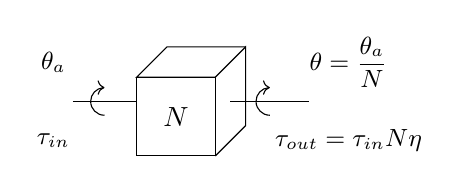
\begin{tikzpicture}
\pgfmathsetmacro{\cubex}{1}
\pgfmathsetmacro{\cubey}{1}
\pgfmathsetmacro{\cubez}{1}
\draw (0,0,0) -- ++(-\cubex,0,0) -- ++(0,-\cubey,0) -- ++(\cubex,0,0) -- cycle;
\draw (0,0,0) -- ++(0,0,-\cubez) -- ++(0,-\cubey,0) -- ++(0,0,\cubez);
\draw (0,0,0) -- ++(-\cubex,0,0) -- ++(0,0,-\cubez) -- ++(\cubex,0,0);
\draw (-2,-.5,-.5) -- ++(.8,0,0) node(a)[midway,above]{} node(b)[midway]{} node(c)[midway,below]{};
\pic [draw,angle radius=5,<-] {angle = a--b--c};
\node at (-2.25,0,-.5) {\small $\theta_a$};
\node at (-2.25,-1,-.5) {\small $\tau_{in}$};
\draw (0,-.5,-.5) -- ++(1,0,0);
\draw (0,-.5,-.5) -- ++(1,0,0) node(a1)[midway,above]{} node(b1)[midway]{} node(c1)[midway,below]{};
\pic [draw,angle radius=5,<-] {angle = a1--b1--c1};
\node at (1.5,0,-.5) {\small $\theta=\dfrac{\theta_a}{N}$};
\node at (1.5,-1,-.5) {\small $\tau_{out}=\tau_{in}N\eta$};
\node at (-.5,-.5,0) {$N$};
\end{tikzpicture}
\end{center}

The motor equation (\ref{eq:motor}) can be expressed in the output coordinates:
\[
Ki_a = J_aN\ddot{\theta} + b_aN\dot{\theta} + \frac{\tau}{N\eta}
\]
Substituing into equation (\ref{eq:va}) and solving for $i_a$:
\[
  i_a = \frac{J_aN}{K}\ddot{\theta} + b_aN\dot{\theta} + \frac{\tau}{N\eta}
\]
\begin{equation}
  V_a = \frac{R_aJ_aN}{K}\ddot{\theta} + \frac{R_ab_aN}{K}\dot{\theta} + \frac{R_a}{KN\eta}\tau + KN\dot{\theta}
  \label{eq:newva}
\end{equation}
Assuming P.D. control, \(V_a = K_p(\theta-\theta_d) + K_d\dot{\theta}\), where $\theta_d$ is the desired orientation of the actuator, the following solution is found by setting the P.D. solution equal to (\ref{eq:newva}). After collecting like terms:

\begin{equation}
  \frac{R_aJ_aN}{K}\ddot{\theta} + \left( \frac{R_aJ_aN}{K} - K_d + KN \right)\dot{\theta} - K_p\theta = -K_p\theta_d - \frac{R_a}{KN\eta}\tau
  \label{eq:end1}
\end{equation}
\newpage
The following parameters of the system can be obtained by applying a step input to the system with $\tau=0$ and measuring the characteristics of it's response. Denoting $\zeta$ as the damping ratio and $\omega_n$ as the natural frequency of the system,
\[
  \text{\% Overshoot} = \left( \frac{\theta_{max} - \theta_{ss}}{\theta_{ss}} \right) \times 100~,\quad \zeta = \frac{-\ln(\sfrac{\%\text{OS}}{100})}{\sqrt{\pi^2 + \ln^2(\sfrac{\%\text{OS}}{100})}}~,\quad \omega_n = \frac{\pi}{T_p\sqrt{1-\zeta^2}}
\]

Given $\theta_{max},~\theta_{ss},$ and $T_p$ as measured parameters of the system's max output, steady state, and time to peak, respectively.

Refactoring equation (\ref{eq:end1}) and equating with the general solution for a second order system given by $\ddot{\theta} + 2\zeta\omega_n\dot{\theta} + \omega_n^2\theta = \omega_n^2\theta_d$,
\begin{equation}
  2\zeta\omega_n = \frac{b_a}{J_a} - \frac{KK_d}{R_aJ_aN} + \frac{K^2}{R_aJ_a}~,\quad
  \omega_n^2 = \frac{-KK_p}{R_aJ_aN}
\end{equation}
Performing a similar experiment as previously described, except with a known inertial load $\tau = J_m\ddot{\theta}$, the following parameters can be found:
\begin{equation}
  \alpha_m \equiv 2\zeta\omega_n = \frac{R_ab_aN^2\eta-KK_dN\eta+K^2N^2\eta}{R_aJ_aN^2\eta+R_aJ_m}~,\quad
  \beta_m \equiv \omega_n =-\frac{KK_pN\eta}{R_aJ_aN^2\eta+R_aJ_m}
\end{equation}

\begin{equation}
\begin{bmatrix}
  1 & -(\alpha_1J_1+\beta_1J_1) \\
  1 & -(\alpha_2J_2+\beta_2J_2) \\
  \vdots & \vdots
\end{bmatrix}
\begin{bmatrix}
  \dfrac{R_ab_aN^2\eta-KK_dN\eta+K^2N^2\eta-KK_pN\eta}{R_aJ_aN^2\eta} \\
  ~\\
  \dfrac{1}{J_aN^2\eta}
\end{bmatrix}
=
\begin{bmatrix}
  \alpha_1+\beta_1 \\
  \alpha_2+\beta_2 \\
  \vdots
\end{bmatrix}
\label{eq:soe}
\end{equation}
Finally, with multiple datasets (varying inertial loads, $J_m$) the coefficients of the second order system equation can be found using the least squares solution of (\ref{eq:soe}).

\newpage
\subsection{ANSYS}
\subsection{Electrical Schematic}
\subsection{Software Flowchart}
\subsection{Project Status and Future}
\subsection{Parts List}



% \begin{enumerate}[label=\alph*.]
%   \item Description for callout a
%   \item Description for callout b
% \end{enumerate}

% Example citations:
% \cite{DBLP:journals/corr/JohnsonAL16}
% \cite{DBLP:journals/corr/abs-1803-09820}
% \cite{DBLP:journals/corr/RonnebergerFB15}

% \newpage
% \bibliographystyle{plain}
% \bibliography{JohnsonAL16,abs-1803-09820,RonnebergerFB15}

\newpage
\section*{Acknowledgements \& Attributions}
We would like to acknowledge the following people for their contibutions to creating this report\textbf{?}
\begin{itemize}
  \item Dr. Isenberg
  \item Dr. Schipper
\end{itemize}

\newpage
\appendix
\renewcommand\thesection{\Roman{section}}
\renewcommand\thesubsection{\roman{subsection}}
\section{Appendix}\label{sec:app}
\begin{figure}[htp]
  \centering
  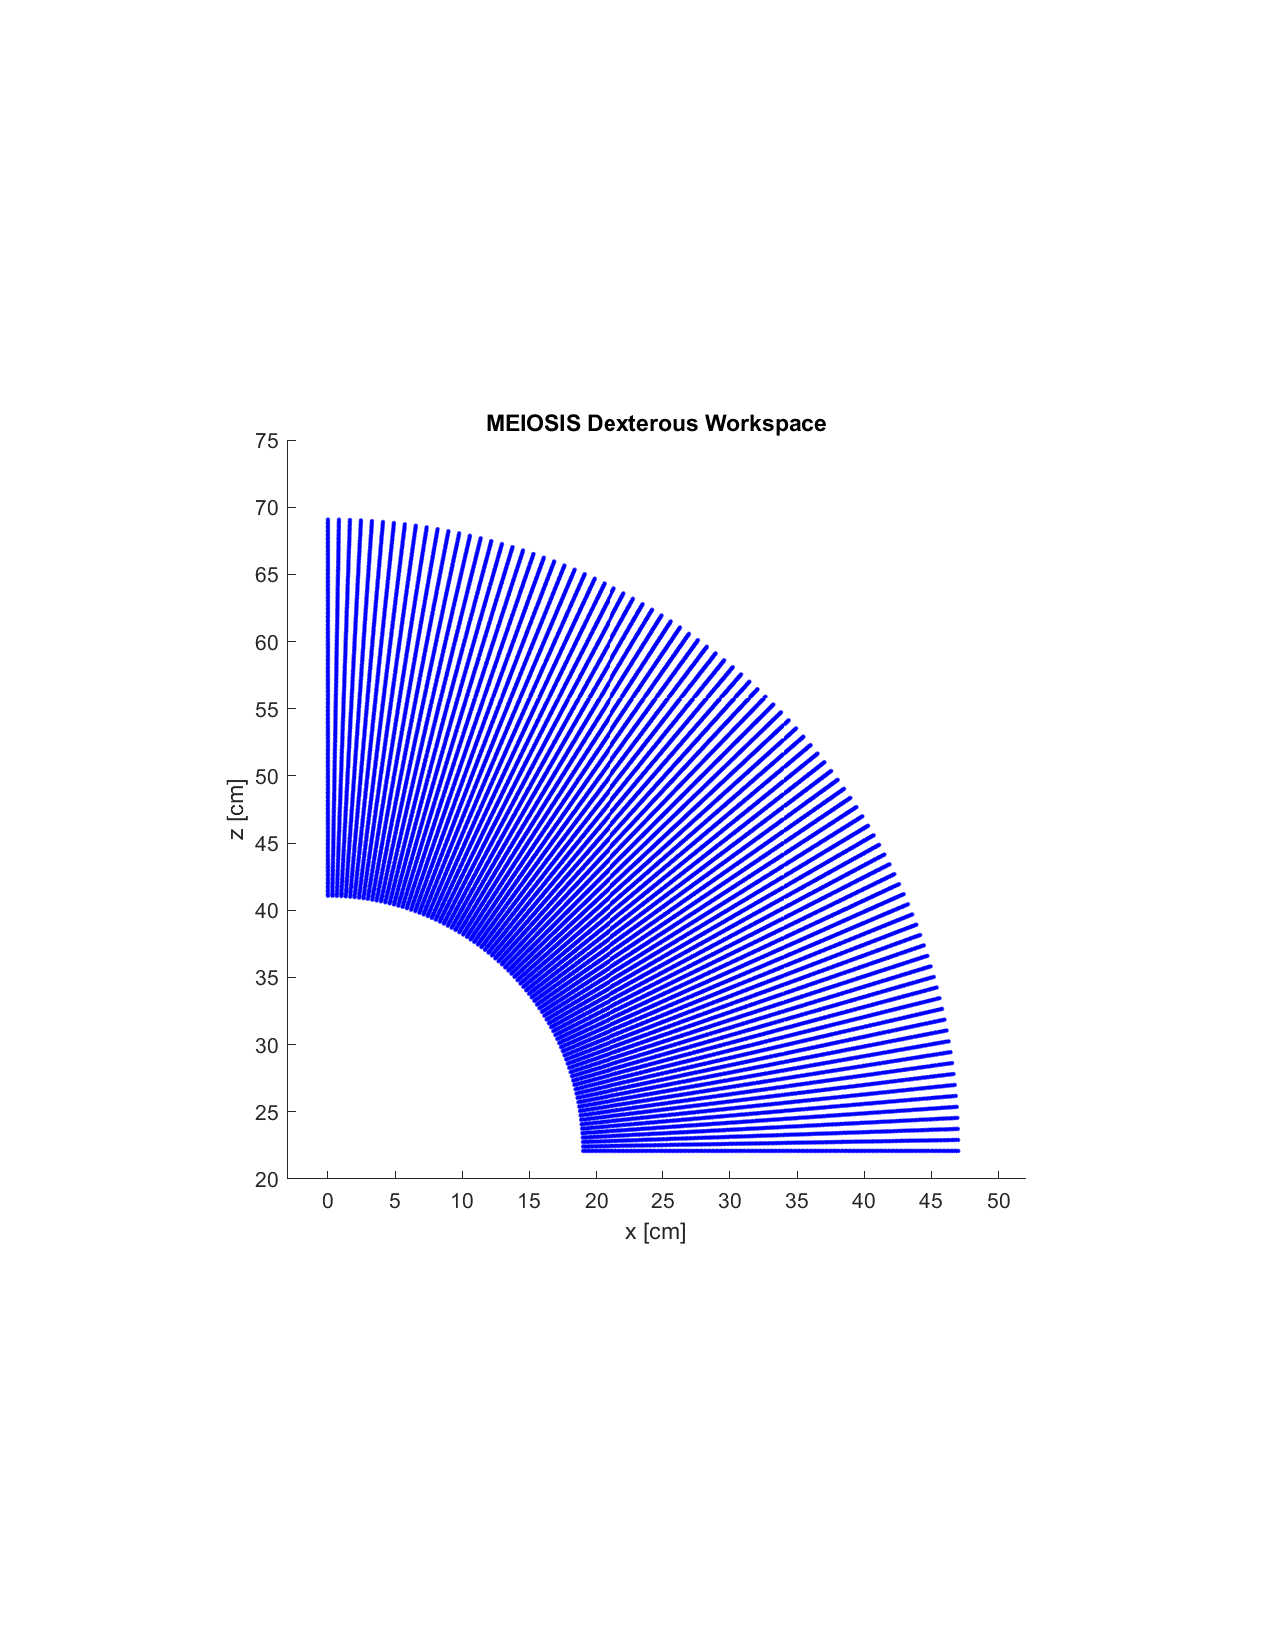
\includegraphics[frame,width=.75\textwidth]{dex}
  \caption{Cross Section of Dexterous Workspace Quadrant}
  \label{fig:dex}
\end{figure}
\subsection{Drawings}
\subsection{Salient Code}
% Code listing
%\begin{lstlisting}[frame=lines,style=Matlab-editor,basicstyle = \mlttfamily, caption=Example Code
% Code Here
%\end{lstlisting}
% \includepdf[landscape,pages=-]{pdfname}

\newpage
\bibliographystyle{plainnat}
\bibliography{robo}

\end{document}
